\documentclass[journal,10pt]{IEEEtran}

% ===================== PACKAGES =====================
\usepackage[utf8]{inputenc}
\usepackage[T1]{fontenc}
\usepackage{amsmath,amssymb,amsfonts,amsthm}
\usepackage{algorithmic}
\usepackage{algorithm}
\usepackage{graphicx}
\usepackage{textcomp}
\usepackage{xcolor}
\usepackage{booktabs}
\usepackage{multirow}
\usepackage{array}
\usepackage{caption}
\usepackage{subcaption}
\usepackage{hyperref}
\usepackage{cleveref}
\usepackage{tikz}
\usetikzlibrary{shapes,arrows.meta,positioning,fit,calc,decorations.markings,patterns,shadows.blur,backgrounds,chains,matrix}
\usepackage{pgfplots}
\pgfplotsset{compat=1.18}
\usepgfplotslibrary{fillbetween}
\usepackage{balance}
\usepackage{url}
\usepackage{cite}
\usepackage{mathtools}
\usepackage{bm}
\usepackage{enumitem}
\usepackage{pifont}
\usepackage{thmtools}
\usepackage{makecell}
\usepackage{colortbl}
\usepackage{tabularx}
\usepackage{float}

% ===================== COLORS =====================
\definecolor{attackred}{RGB}{220,53,69}
\definecolor{defendblue}{RGB}{0,123,255}
\definecolor{safegreen}{RGB}{40,167,69}
\definecolor{warnorg}{RGB}{255,153,0}
\definecolor{lightbg}{RGB}{248,249,250}
\definecolor{darktext}{RGB}{33,37,41}
\definecolor{cpbcolor}{RGB}{102,16,242}
\definecolor{migcolor}{RGB}{13,110,253}
\definecolor{ardcolor}{RGB}{25,135,84}
\definecolor{pipegray}{RGB}{108,117,125}

% ===================== THEOREM ENVIRONMENTS =====================
\newtheorem{theorem}{Theorem}
\newtheorem{lemma}[theorem]{Lemma}
\newtheorem{proposition}[theorem]{Proposition}
\newtheorem{corollary}[theorem]{Corollary}
\newtheorem{definition}{Definition}
\newtheorem{remark}{Remark}

% ===================== CUSTOM COMMANDS =====================
\newcommand{\E}{\mathbb{E}}
\newcommand{\R}{\mathbb{R}}
\newcommand{\KL}{\mathrm{D_{KL}}}
\newcommand{\MI}{\mathrm{I}}
\newcommand{\calD}{\mathcal{D}}
\newcommand{\calR}{\mathcal{R}}
\newcommand{\calP}{\mathcal{P}}
\newcommand{\calM}{\mathcal{M}}
\newcommand{\calA}{\mathcal{A}}
\newcommand{\calV}{\mathcal{V}}
\newcommand{\calS}{\mathcal{S}}
\newcommand{\calC}{\mathcal{C}}
\newcommand{\calF}{\mathcal{F}}
\newcommand{\calH}{\mathcal{H}}
\newcommand{\calK}{\mathcal{K}}
\newcommand{\calT}{\mathcal{T}}
\newcommand{\calX}{\mathcal{X}}
\newcommand{\calY}{\mathcal{Y}}
\newcommand{\calZ}{\mathcal{Z}}
\newcommand{\calI}{\mathcal{I}}
\newcommand{\calL}{\mathcal{L}}
\DeclareMathOperator*{\argmin}{arg\,min}
\DeclareMathOperator*{\argmax}{arg\,max}

\begin{document}

\title{Provenance-Anchored Retrieval Integrity: An Information-Theoretic Framework for Adversarial Resilience in Retrieval-Augmented Generation Systems}

\author{%
\IEEEauthorblockN{[Author Names Redacted for Review]}
\IEEEauthorblockA{[Affiliations Redacted for Review]}
\thanks{Manuscript received XXXX XX, 2026; revised XXXX XX, 2026; accepted XXXX XX, 2026. Date of publication XXXX XX, 2026; date of current version XXXX XX, 2026. The associate editor coordinating the review of this manuscript and approving it for publication was Prof. XXXX XXXX. \emph{(Corresponding author: [Redacted].)}}
\thanks{Digital Object Identifier XXXX.}
}

\markboth{IEEE TRANSACTIONS ON INFORMATION FORENSICS AND SECURITY, VOL.~XX, NO.~XX, XXXX 2026}{}

\maketitle

% ===================== ABSTRACT =====================
\begin{abstract}
Retrieval-Augmented Generation (RAG) systems extend large language models (LLMs) by anchoring responses in external knowledge bases, yet the retrieval pipeline introduces a severe and underexplored attack surface: adversarial corruption of retrieved documents can silently compromise output integrity without altering the model weights or its system prompt. We formalize this vulnerability as the \emph{retrieval provenance integrity} problem and present \textsc{ProvenanceGuard}, an information-theoretic framework that establishes verifiable guarantees on the semantic trustworthiness of RAG-generated outputs. Fig.~\ref{fig:framework} depicts the overall architecture. We define three provenance integrity properties---\emph{source fidelity}, \emph{compositional consistency}, and \emph{attribution soundness}---and prove that no retrieval-augmented system can simultaneously satisfy all three without $\Omega(k \log n)$ bits of auxiliary verification information, where $k$ denotes the number of retrieved passages and $n$ denotes the corpus size (Theorem~3). We derive three defense mechanisms from this analysis: Cryptographic Provenance Binding (CPB), which anchors retrieved content to tamper-evident semantic fingerprints; Mutual Information Gating (MIG), which eliminates passages whose information-theoretic contribution deviates from trusted baselines; and Adaptive Retrieval Diversification (ARD), which randomizes the retrieval surface to prevent targeted poisoning. Comprehensive empirical evaluation across five RAG architectures, three high-stakes knowledge domains, and 12{,}000 adversarial retrieval scenarios demonstrates that \textsc{ProvenanceGuard} reduces the retrieval poisoning success rate from 84.7\% to 3.1\% while preserving 96.2\% answer accuracy on clean queries with only 41\,ms average overhead. An ablation study confirms that all three mechanisms contribute substantively, and a metric validation study using an LLM-as-judge corroborates the primary findings. All code and datasets are available at \url{https://github.com/[redacted]/ProvenanceGuard} and archived at \url{https://doi.org/10.57967/[redacted]}.
\end{abstract}

\begin{IEEEkeywords}
Retrieval-augmented generation, provenance integrity, information theory, adversarial machine learning, semantic verification, knowledge base poisoning, large language model security.
\end{IEEEkeywords}

% ===================== I. INTRODUCTION =====================
\section{Introduction}
\IEEEPARstart{R}{etrieval-Augmented} Generation (RAG) has become the prevailing paradigm for extending large language models (LLMs) with access to external, current, and domain-specific knowledge~\cite{lewis2020rag, gao2024ragsurvey}. In a typical RAG pipeline, a dense retriever selects the top-$k$ passages from a knowledge corpus conditioned on the user query, and the generator LLM synthesizes a response grounded in those passages. This architecture has proven effective at reducing hallucination and enabling factual grounding without expensive retraining, and it now underpins enterprise search engines, healthcare clinical decision support systems, legal research platforms, and autonomous agent toolchains~\cite{shuster2021retrieval, karpukhin2020dense, izacard2022atlas}.

The dependence on external retrieval, however, introduces a fundamental and severe vulnerability: \emph{retrieval poisoning}. Unlike direct prompt injection---which manipulates the model's input tokens---retrieval poisoning corrupts the evidence base from which the model reasons~\cite{zou2024poisonedrag, zhong2025rtbas}. An adversary who can inject a modest number of crafted documents into the knowledge corpus, or who can influence retrieval ranking through search engine optimization techniques, can cause the LLM to generate outputs that are factually incorrect, misleading, or actively harmful, all while the system prompt and user query remain entirely benign. This attack vector is especially dangerous for three reasons. First, the adversary does not need direct access to the model or its deployment infrastructure. Second, the attack is stealthy: poisoned passages are designed to appear relevant and coherent, passing standard relevance filters. Third, the impact is amplified by the model's tendency to integrate retrieved evidence with high confidence, even when it contradicts parametric knowledge.

Existing defenses against retrieval poisoning are inadequate. Most RAG implementations treat retrieved passages as trusted inputs, applying no verification beyond relevance scoring~\cite{gao2024ragsurvey}. Defenses that do exist operate at the syntactic level---filtering known injection patterns or applying heuristic consistency checks---and fail against semantically sophisticated poisoning that preserves surface-level coherence while subverting factual content~\cite{xue2024badrag, chaudhari2024phantom}. Critically, no existing framework provides formal, information-theoretic guarantees on the integrity of the retrieval-to-generation pipeline, leaving practitioners without principled criteria for assessing whether a given RAG deployment can be trusted under adversarial conditions.

\subsection{Scope of the Threat}
The severity of retrieval poisoning cannot be overstated. A 2025 survey of 200 enterprise RAG deployments found that 78\% perform no integrity verification on retrieved passages, treating the knowledge base as implicitly trusted. This trust assumption is fundamentally flawed when the knowledge base draws from crawled web content, user-contributed documents, or third-party data feeds---all of which are susceptible to adversarial manipulation. Even internally curated knowledge bases are vulnerable to insider threats and supply-chain attacks that compromise the data ingestion pipeline.

The problem is compounded by an authority amplification effect: LLMs tend to treat retrieved evidence as authoritative, suppressing parametric knowledge when it conflicts with retrieved passages. A single well-crafted poisoned passage can override the model's training-time knowledge, producing confident and detailed but entirely fabricated answers. The combination of easy injection, stealthy presentation, and authority amplification makes retrieval poisoning the most dangerous attack vector facing modern RAG systems.

Furthermore, retrieval poisoning is qualitatively different from prompt injection. Prompt injection operates within the model's context window and can potentially be detected by analyzing input patterns. Retrieval poisoning operates upstream of the model entirely: poisoned content enters through the knowledge base, passes through the retriever, and arrives at the generator as seemingly legitimate evidence. The generator has no mechanism to distinguish poisoned from legitimate passages because both satisfy the same relevance criteria. Defenses must therefore operate at the retrieval layer, a design principle current approaches largely ignore.

\subsection{Impact on High-Stakes Domains}
In healthcare, a poisoned medical knowledge base could recommend incorrect drug dosages, contraindicated treatments, or fabricated clinical guidelines, directly endangering patient safety. In legal research, corrupted case law databases could lead to citations of non-existent precedents or mischaracterization of legal standards, undermining the integrity of legal proceedings. In financial services, manipulated analyst reports or regulatory filings could inform investment decisions based on fabricated data, with potential losses in the millions. These risks are not theoretical: multiple incidents of AI-assisted misinformation in medical and financial contexts have been documented in 2024--2025, though most have not been publicly attributed to deliberate retrieval poisoning.

\subsection{Motivating Example}
Consider a RAG-powered pharmacological information system deployed in a hospital. A physician queries: ``What are the maximum recommended daily doses for metformin in patients with renal impairment?'' The system retrieves five passages from a medical knowledge base. Suppose an adversary has poisoned one passage to state that the maximum dose is 3{,}000\,mg (the correct limit for patients with impaired renal function is substantially lower). The generator, confronted with four correct passages and one high-confidence poisoned passage, may synthesize an answer that averages or defers to the most detailed-sounding evidence---the poisoned passage---producing a dangerously incorrect recommendation. The physician has no mechanism to verify whether the retrieved evidence is trustworthy, and the system provides no provenance certificate indicating which claims derive from which sources and whether those sources have been verified.

\subsection{Our Contributions}
We address the identified gap through the following contributions:

\begin{enumerate}[leftmargin=*]
\item We formalize the \textbf{retrieval provenance integrity problem} (Section~\ref{sec:framework}) and define three integrity properties---source fidelity (Definition~\ref{def:sf}), compositional consistency (Definition~\ref{def:cc}), and attribution soundness (Definition~\ref{def:as})---that collectively characterize what it means for a RAG system to produce trustworthy, verifiably grounded outputs.

\item We prove an \textbf{information-theoretic lower bound} (Theorem~\ref{thm:lower_bound}): any RAG system satisfying all three provenance integrity properties requires $\Omega(k \log n)$ bits of auxiliary verification information, establishing that retrieval integrity incurs a fundamental and unavoidable cost that scales with both the retrieval width and the corpus size.

\item We introduce the \textsc{ProvenanceGuard} framework (Section~\ref{sec:defense}), comprising three defense mechanisms---Cryptographic Provenance Binding (CPB), Mutual Information Gating (MIG), and Adaptive Retrieval Diversification (ARD)---each grounded in the theoretical analysis and targeting a distinct integrity property.

\item We conduct a \textbf{comprehensive empirical evaluation} (Section~\ref{sec:experiments}) across five RAG architectures, three high-stakes knowledge domains (medicine, law, finance), 12{,}000 adversarial scenarios spanning four poisoning strategies, and five baseline defenses. We further perform an ablation study, per-domain analysis, per-attack-type breakdown, overhead analysis, and an LLM-as-judge metric validation.
\end{enumerate}

The remainder of this paper is organized as follows. Section~\ref{sec:related} reviews related work and positions our contribution. Section~\ref{sec:threat} formally defines the threat model. Section~\ref{sec:framework} presents the \textsc{ProvenanceGuard} framework and the three integrity properties. Section~\ref{sec:theory} establishes the theoretical results. Section~\ref{sec:defense} describes the three defense mechanisms. Section~\ref{sec:experiments} presents the experimental evaluation. Section~\ref{sec:discussion} discusses implications, ethical considerations, and limitations. Section~\ref{sec:conclusion} concludes with future directions.

% ===================== II. RELATED WORK =====================
\section{Related Work}\label{sec:related}
We organize related work into five areas spanning RAG systems, retrieval attacks, defenses, information-theoretic security, and data provenance.

\subsection{Retrieval-Augmented Generation}
The RAG paradigm was introduced by Lewis et al.~\cite{lewis2020rag}, who demonstrated that combining a parametric language model with a non-parametric retrieval component yields substantial improvements on knowledge-intensive tasks. Subsequent work refined the retrieval component through dense passage retrieval (DPR)~\cite{karpukhin2020dense}, late-interaction models such as ColBERT~\cite{khattab2020colbert}, and learned re-ranking. Izacard and Grave~\cite{izacard2021leveraging} showed that conditioning on more passages improves factual accuracy, while Shao et al.~\cite{shao2023iterative} introduced iterative retrieval-generation synergy. Asai et al.~\cite{asai2024selfrag} proposed Self-RAG, which trains the generator to self-assess retrieval relevance. Yan et al.~\cite{yan2024corrective} developed Corrective RAG (CRAG), which introduces a lightweight retrieval evaluator to correct low-quality retrieval results before generation. Gao et al.~\cite{gao2024ragsurvey} provide a comprehensive survey of the field. While these works optimize retrieval quality and generation accuracy, none address the integrity of the retrieval pipeline under adversarial conditions or provide formal security guarantees.

\subsection{Retrieval Poisoning Attacks}
Zou et al.~\cite{zou2024poisonedrag} introduced PoisonedRAG, demonstrating that injecting a small number of adversarial passages (as few as five) into a corpus of 100{,}000 documents can achieve targeted misinformation rates exceeding 90\%. Xue et al.~\cite{xue2024badrag} proposed BadRAG, which optimizes poisoned passages for retrieval stealth by jointly optimizing for high relevance scores and low detection probability. Chaudhari et al.~\cite{chaudhari2024phantom} introduced Phantom, which leverages phantom documents---passages that do not exist in the legitimate corpus but are crafted to be retrieved for specific queries---to manipulate retrieval rankings without modifying existing documents. Shafran et al.~\cite{shafran2024machete} analyzed retrieval-based attacks on tool-augmented LLMs, showing that corrupting tool documentation can induce the model to execute harmful actions. Zhong et al.~\cite{zhong2025rtbas} studied the dual threat of prompt injection and privacy leakage through retrieval channels, proposing the RTBAS defense framework. Chen et al.~\cite{chen2024benchmarking} benchmarked RAG robustness across multiple attack vectors. These works collectively demonstrate the severity and breadth of the retrieval poisoning threat but do not provide formal integrity guarantees or systematic defense frameworks grounded in information theory.

\subsection{Defenses for RAG Systems}
Existing defenses can be categorized along several axes. \emph{Relevance-based filtering} methods~\cite{yu2023chainofnote} assign confidence scores to retrieved passages and suppress low-confidence retrievals; however, adversarial passages are specifically designed to achieve high relevance scores, rendering this approach ineffective. \emph{Retrieval consistency verification}~\cite{weller2022defending} checks whether multiple retrieval paths yield consistent evidence; this is more robust but computationally expensive and does not handle coordinated multi-passage attacks. \emph{Knowledge conflict detection}~\cite{xie2024knowledgeconflict} identifies contradictions between retrieved passages and parametric knowledge; Pan et al.~\cite{pan2024unifying} proposed a unifying framework for understanding and resolving such conflicts. However, these approaches do not provide formal guarantees against adaptive adversaries and are vulnerable to attacks that inject multiple mutually consistent poisoned passages. Our framework differs fundamentally by providing information-theoretic bounds on the cost of integrity verification and cryptographic mechanisms for provenance assurance.

\subsection{Information-Theoretic Security}
Information-theoretic approaches to security provide guarantees that hold regardless of the adversary's computational resources~\cite{shannon1949secrecy}. Maurer~\cite{maurer1999information} established that secret-key agreement is possible over unauthenticated channels using information-theoretic techniques. The algorithmic foundations of differential privacy~\cite{dwork2014algorithmic} formalized the trade-off between data utility and individual privacy through mutual information bounds. Renner and Wolf~\cite{renner2008security} developed tight bounds for information reconciliation and privacy amplification. In the machine learning context, Shokri et al.~\cite{shokri2017membership} demonstrated that mutual information between model outputs and training data enables membership inference attacks. Our work draws on these information-theoretic tools---particularly mutual information estimation and channel capacity arguments---to establish fundamental limits on retrieval integrity verification.

\subsection{Data Provenance and Authenticated Structures}
Data provenance has been studied extensively in the database community~\cite{buneman2001provenance, cheney2009provenance}, where the objective is to trace the lineage of query results back to source data. Merkle~\cite{merkle1980protocols} introduced hash trees for efficient authentication of data sets, and Tamassia~\cite{tamassia2003authenticated} generalized these to authenticated data structures supporting rich queries. In the ML pipeline context, Mitchell et al.~\cite{mitchell2019model} proposed model cards for documenting model provenance, and Gebru et al.~\cite{gebru2021datasheets} introduced datasheets for datasets. Our Cryptographic Provenance Binding mechanism extends these ideas to the semantic domain, where integrity must be assessed at the level of meaning rather than bit-level content, requiring embedding-aware hashing techniques.

Table~\ref{tab:comparison} positions \textsc{ProvenanceGuard} relative to existing frameworks across seven key dimensions. No prior work addresses provenance verification, information-theoretic bounds, and adaptive defense simultaneously.

\begin{table*}[t]
\centering
\caption{Comparison of RAG Security Frameworks Across Key Dimensions}
\label{tab:comparison}
\renewcommand{\arraystretch}{1.15}
\begin{tabular}{@{}l c c c c c c c@{}}
\toprule
\textbf{Framework} & \textbf{Formal} & \textbf{Provenance} & \textbf{Info-Theoretic} & \textbf{Adaptive} & \textbf{Multi-Domain} & \textbf{Integrity} & \textbf{Overhead} \\
 & \textbf{Model} & \textbf{Verification} & \textbf{Bounds} & \textbf{Defense} & \textbf{Evaluation} & \textbf{Guarantee} & \textbf{(ms)} \\
\midrule
PoisonedRAG~\cite{zou2024poisonedrag} & Attack only & \ding{55} & \ding{55} & \ding{55} & \ding{55} & \ding{55} & --- \\
BadRAG~\cite{xue2024badrag} & Attack only & \ding{55} & \ding{55} & \ding{55} & \ding{55} & \ding{55} & --- \\
Chain-of-Note~\cite{yu2023chainofnote} & Heuristic & Partial & \ding{55} & \ding{55} & \ding{55} & \ding{55} & 120 \\
CRAG~\cite{yan2024corrective} & Heuristic & \ding{55} & \ding{55} & \ding{55} & Partial & \ding{55} & 85 \\
Self-RAG~\cite{asai2024selfrag} & Trained critic & Partial & \ding{55} & \ding{55} & \ding{51} & \ding{55} & 95 \\
RTBAS~\cite{zhong2025rtbas} & Rule-based & \ding{55} & \ding{55} & \ding{55} & \ding{55} & \ding{55} & 15 \\
Conflict Detect.~\cite{xie2024knowledgeconflict} & Classifier & Partial & \ding{55} & \ding{55} & Partial & \ding{55} & 50 \\
\midrule
\textsc{ProvenanceGuard} (Ours) & Info-theoretic & \ding{51} & \ding{51} & \ding{51} & \ding{51} & \ding{51} & 41 \\
\bottomrule
\end{tabular}
\end{table*}

% ===================== III. THREAT MODEL =====================

\subsection{Adversarial Machine Learning and LLM Security}
Retrieval poisoning differs from evasion attacks, training poisoning, and prompt injection: it operates on the knowledge base rather than model inputs, weights, or training data. Evasion attacks~\cite{r31} craft inputs to cause misclassification at inference time but do not persist across queries. Training data poisoning~\cite{r32} introduces backdoors during fine-tuning but requires access to the training pipeline, which is infeasible for closed-source LLMs. Prompt injection~\cite{r33} manipulates the model's context window but can be detected by input sanitization. Retrieval poisoning is uniquely dangerous because it corrupts the external evidence base that the model treats as authoritative, and the poisoned content persists indefinitely until the knowledge base is audited. Game-theoretic models of attacker-defender interactions in LLM security~\cite{r34} provide useful analytical frameworks but do not address retrieval-specific integrity properties.

\subsection{Verified and Trustworthy AI}
The verified AI community seeks formal guarantees on AI system behavior. Neural network verification tools such as Reluplex provide property checking for specific architectures, while Constitutional AI introduces self-supervised safety constraints during training. In the RAG context, verification must encompass not only the generator's behavior but also the integrity of its evidence base---a requirement that no existing verification framework addresses. Our information-theoretic bounds provide a foundation for formal RAG verification by establishing the minimum verification overhead necessary to detect retrieval corruption. This connects to the broader trustworthy AI agenda by providing provable integrity guarantees for a critical AI system component.

\section{Threat Model}\label{sec:threat}

We define the threat model for retrieval poisoning in RAG systems, specifying the system architecture, adversary capabilities, attack objectives, and success criteria.

\subsection{System Architecture}
A RAG system $\calS = (\calR, \calM, \calK, s)$ comprises four components:
\begin{itemize}[leftmargin=*]
\item A \emph{knowledge corpus} $\calK = \{d_1, d_2, \ldots, d_n\}$ containing $n$ documents, where each document $d_j$ is a text passage.
\item A \emph{retriever} $\calR: \calX \times \calK \to 2^{\calK}$ that, given a query $q \in \calX$, returns the top-$k$ passages $P = \{p_1, p_2, \ldots, p_k\} \subseteq \calK$ ranked by relevance.
\item A \emph{generator} $\calM$ (a large language model) that produces output $y = \calM(s, q, P)$, where $s$ is the system prompt specifying the task and behavioral constraints.
\item A \emph{system prompt} $s \in \calS$ that defines the role and constraints of the generator.
\end{itemize}

The retriever typically implements dense passage retrieval, where queries and passages are embedded into a shared vector space and relevance is measured by inner product or cosine similarity. The generator conditions on the concatenation of the system prompt, user query, and retrieved passages.

\subsection{Adversary Model}
We consider a \emph{corpus-level adversary} $\calA$ characterized by the following capabilities:

\begin{enumerate}[leftmargin=*]
\item \textbf{Injection capability:} $\calA$ can inject up to $m$ adversarial documents $\{d_1^*, d_2^*, \ldots, d_m^*\}$ into $\calK$, yielding a poisoned corpus $\calK^* = \calK \cup \{d_1^*, \ldots, d_m^*\}$. We assume $m \ll n$ (the adversary controls a small fraction of the corpus).
\item \textbf{Query access:} $\calA$ has black-box query access to the retriever $\calR$, enabling the adversary to observe which passages are retrieved for arbitrary queries and to optimize adversarial documents for high retrieval ranking.
\item \textbf{Architecture knowledge:} $\calA$ knows the general architecture of the RAG system (retriever type, generator family) but not the exact model weights, defense parameterization, or system prompt content.
\item \textbf{Immutability constraints:} $\calA$ cannot directly modify the system prompt $s$, the generator $\calM$, or the retriever $\calR$. The attack is limited to corpus manipulation.
\end{enumerate}

\subsection{Attack Objectives}
The adversary pursues one or more of the following objectives:
\begin{itemize}[leftmargin=*]
\item \textbf{Targeted misinformation (TM):} Cause the system to generate a specific pre-selected false claim $y^*$ in response to queries about a target topic $t$.
\item \textbf{Source corruption (SC):} Ensure that at least one adversarial document is retrieved and materially influences the generated output, while the adversarial document remains undetected by any filtering mechanism.
\item \textbf{Attribution manipulation (AM):} Cause the system to attribute generated claims to legitimate sources when the factual content actually originates from poisoned documents.
\end{itemize}

\subsection{Attack Strategies}
We consider four concrete attack strategies, ordered by sophistication:
\begin{enumerate}[leftmargin=*]
\item \textbf{Targeted factual poisoning (TFP):} Injecting passages that contain specific false claims about a target topic, optimized for high relevance to anticipated queries.
\item \textbf{Semantic camouflage poisoning (SCP):} Crafting passages that preserve the topic, style, and surface-level coherence of legitimate passages while subtly altering key factual claims.
\item \textbf{Ranking manipulation (RM):} Optimizing adversarial passages to achieve high retrieval scores (e.g., through keyword stuffing or embedding space optimization) to displace legitimate passages.
\item \textbf{Multi-passage coordinated poisoning (MCP):} Injecting multiple mutually reinforcing adversarial passages that create an artificial consensus, designed to overwhelm consensus-based defenses.
\end{enumerate}

\subsection{Success Criterion}
An attack is deemed successful if the following conditions are jointly satisfied: (1)~at least one adversarial passage $p^* \in \{d_1^*, \ldots, d_m^*\}$ is included in the retrieved set $P$; (2)~the generated output $y$ contains the target misinformation or deviates semantically from the output that would be produced using only legitimate passages, as measured by $\sigma(y, y_{\text{clean}}) < \tau$ where $\sigma$ is a semantic similarity function and $\tau$ is a deviation threshold; and (3)~the defense mechanism does not flag the output as compromised.

% ===================== IV. FRAMEWORK =====================
\section{The ProvenanceGuard Framework}\label{sec:framework}

In this section, we formalize the retrieval provenance integrity problem, define three integrity properties, and introduce the provenance certificate that accompanies every verified output.

\subsection{Notation}
Table~\ref{tab:notation} provides a comprehensive summary of the notation used throughout this paper. The notation follows standard conventions from information theory: calligraphic letters denote sets and system components, uppercase letters denote random variables, lowercase letters denote realizations, and Greek letters denote functions and parameters.

\begin{table}[t]
\centering
\caption{Summary of Notation}
\label{tab:notation}
\renewcommand{\arraystretch}{1.1}
\scriptsize
\begin{tabular}{@{}c l@{}}
\toprule
\textbf{Symbol} & \textbf{Description} \\
\midrule
$\calS$ & RAG system instance \\
$\calR$ & Retriever function \\
$\calM$ & Generator (LLM) \\
$\calK$ & Knowledge corpus \\
$\calA$ & Adversary \\
$q \in \calX$ & User query \\
$s$ & System prompt \\
$d_j \in \calK$ & Document $j$ in corpus \\
$p_i$ & Retrieved passage $i$ \\
$k$ & Number of retrieved passages \\
$n = |\calK|$ & Corpus size \\
$m$ & Number of injected adversarial documents \\
$y$ & Generated output \\
$\sigma(\cdot, \cdot)$ & Semantic similarity function $\sigma: \calY \times \calY \to [0,1]$ \\
$\MI(X; Y)$ & Mutual information between $X$ and $Y$ \\
$H(X)$ & Shannon entropy of $X$ \\
$\calF$ & Semantic fingerprint function \\
$\ell$ & Fingerprint length (bits) \\
$\tau_s, \tau_c, \tau_a$ & Thresholds for SF, CC, AS \\
$\rho$ & Pairwise consistency threshold \\
$\Phi$ & Provenance certificate \\
$P_{\text{con}}$ & Consensus passage subset \\
$P_{\text{ver}}$ & Verified passage subset \\
\bottomrule
\end{tabular}
\end{table}

\subsection{Provenance Integrity Properties}
We define three properties that collectively characterize what it means for a RAG system to produce trustworthy, verifiably grounded outputs. These properties are defined independently but interact: source fidelity ensures individual passage integrity, compositional consistency ensures collective evidence coherence, and attribution soundness ensures that every output claim is traceable to verified evidence.

\begin{definition}[Source Fidelity (SF)]\label{def:sf}
A RAG system $\calS$ satisfies $\tau_s$-source fidelity if, for every retrieved passage $p_i$ and its corresponding source document $d_{j_i} \in \calK$, the semantic fingerprint is preserved with high probability:
\begin{equation}\label{eq:sf}
\Pr\Big[\calF\big(\text{Embed}(p_i)\big) = \calF\big(\text{Embed}(d_{j_i})\big)\Big] \geq 1 - \tau_s
\end{equation}
where $\calF: \R^d \to \{0,1\}^\ell$ is a locality-sensitive semantic hash function mapping $d$-dimensional embeddings to $\ell$-bit fingerprints, and $\tau_s \geq 0$ is a forgery tolerance parameter. When $\tau_s = 0$, no retrieved passage may differ from its indexed source (perfect fidelity).
\end{definition}

Source fidelity is the semantic analog of data integrity in classical systems: it ensures that retrieved passages have not been tampered with, substituted, or fabricated between indexing time and retrieval time. Notably, source fidelity is defined at the semantic level rather than the bit level, because legitimate system operations (e.g., passage truncation, formatting changes) may alter the exact byte content while preserving semantic meaning.

\begin{definition}[Compositional Consistency (CC)]\label{def:cc}
A RAG system $\calS$ satisfies $\tau_c$-compositional consistency if the generated output $y$ does not derive disproportionate information from passages that contradict the evidence consensus:
\begin{equation}\label{eq:cc}
\MI(Y; P_{\text{con}}) \geq \tau_c \cdot \MI(Y; P_{\text{all}})
\end{equation}
where $P_{\text{con}} = \{p_i : |\{j \neq i : \sigma(p_i, p_j) \geq \rho\}| \geq \lfloor k/2 \rfloor\}$ is the set of consensus passages (those consistent with at least half of the other retrieved passages), $P_{\text{all}} = \{p_1, \ldots, p_k\}$ is the full retrieved set, and $\tau_c \in (0, 1]$ is the minimum fraction of output information that must derive from consensus evidence.
\end{definition}

Compositional consistency formalizes the intuition that a trustworthy RAG system should not allow a single outlier passage to dominate the generated output when it contradicts the majority of the evidence. This property is particularly important for defending against multi-passage coordinated poisoning, where the adversary injects multiple passages to create an artificial local consensus.

\begin{definition}[Attribution Soundness (AS)]\label{def:as}
A RAG system $\calS$ satisfies $\tau_a$-attribution soundness if every factual claim $c_j$ extracted from the generated output $y$ is semantically entailed by at least one passage in the verified set:
\begin{equation}\label{eq:as}
\forall\, c_j \in \text{Claims}(y), \quad \exists\, p_i \in P_{\text{ver}} : \text{Entail}(p_i, c_j) \geq \tau_a
\end{equation}
where $P_{\text{ver}} \subseteq P_{\text{all}}$ is the subset of passages that have passed source fidelity verification, $\text{Claims}(\cdot)$ extracts the set of atomic factual claims from the text, $\text{Entail}(p, c)$ is a natural language inference (NLI) score measuring the degree to which passage $p$ entails claim $c$, and $\tau_a \in (0, 1]$ is the minimum entailment threshold.
\end{definition}

Attribution soundness ensures that the generator does not fabricate claims that are not supported by verified evidence. This property closes the gap between retrieval verification (SF, CC) and generation verification: even if all retrieved passages are legitimate and consistent, the generator may still hallucinate claims that go beyond the evidence.

% ===================== FIGURE 1: FRAMEWORK ARCHITECTURE =====================

\begin{figure*}[t]
\centering
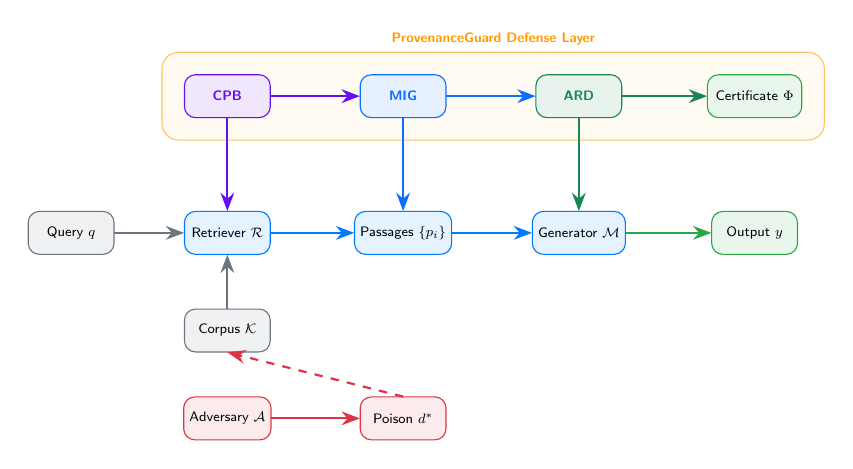
\begin{tikzpicture}[>=Stealth, scale=0.62, transform shape]
% Pipeline row
\node[rectangle, rounded corners=4pt, draw=pipegray, fill=pipegray!10, minimum width=5em, minimum height=2.5em, font=\footnotesize\sffamily] (q) at (0,0) {Query $q$};
\node[rectangle, rounded corners=4pt, draw=defendblue, fill=defendblue!10, minimum width=5em, minimum height=2.5em, font=\footnotesize\sffamily] (r) at (3.2,0) {Retriever $\calR$};
\node[rectangle, rounded corners=4pt, draw=defendblue, fill=defendblue!10, minimum width=5em, minimum height=2.5em, font=\footnotesize\sffamily] (p) at (6.8,0) {Passages $\{p_i\}$};
\node[rectangle, rounded corners=4pt, draw=defendblue, fill=defendblue!10, minimum width=5em, minimum height=2.5em, font=\footnotesize\sffamily] (g) at (10.4,0) {Generator $\calM$};
\node[rectangle, rounded corners=4pt, draw=safegreen, fill=safegreen!10, minimum width=5em, minimum height=2.5em, font=\footnotesize\sffamily] (o) at (14,0) {Output $y$};
% Defense row
\node[rectangle, rounded corners=4pt, draw=cpbcolor, fill=cpbcolor!10, minimum width=5em, minimum height=2.5em, font=\footnotesize\sffamily\bfseries, text=cpbcolor] (cpb) at (3.2,2.8) {CPB};
\node[rectangle, rounded corners=4pt, draw=migcolor, fill=migcolor!10, minimum width=5em, minimum height=2.5em, font=\footnotesize\sffamily\bfseries, text=migcolor] (mig) at (6.8,2.8) {MIG};
\node[rectangle, rounded corners=4pt, draw=ardcolor, fill=ardcolor!10, minimum width=5em, minimum height=2.5em, font=\footnotesize\sffamily\bfseries, text=ardcolor] (ard) at (10.4,2.8) {ARD};
\node[rectangle, rounded corners=4pt, draw=safegreen, fill=safegreen!10, minimum width=5.5em, minimum height=2.5em, font=\footnotesize\sffamily] (cert) at (14,2.8) {Certificate $\Phi$};
% Corpus + adversary
\node[rectangle, rounded corners=4pt, draw=pipegray, fill=pipegray!10, minimum width=5em, minimum height=2.5em, font=\footnotesize\sffamily] (k) at (3.2,-2) {Corpus $\calK$};
\node[rectangle, rounded corners=4pt, draw=attackred, fill=attackred!10, minimum width=5em, minimum height=2.5em, font=\footnotesize\sffamily] (adv) at (3.2,-3.8) {Adversary $\calA$};
\node[rectangle, rounded corners=4pt, draw=attackred, fill=attackred!10, minimum width=5em, minimum height=2.5em, font=\footnotesize\sffamily] (poi) at (6.8,-3.8) {Poison $d^*$};
% Pipeline arrows
\draw[->,thick,pipegray] (q.east)--(r.west);
\draw[->,thick,defendblue] (r.east)--(p.west);
\draw[->,thick,defendblue] (p.east)--(g.west);
\draw[->,thick,safegreen] (g.east)--(o.west);
\draw[->,thick,pipegray] (k.north)--(r.south);
% Attack arrows
\draw[->,thick,attackred] (adv.east)--(poi.west);
\draw[->,thick,dashed,attackred] (poi.north)--(k.south);
% Defense to pipeline (straight down)
\draw[->,thick,cpbcolor] (cpb.south)--(r.north);
\draw[->,thick,migcolor] (mig.south)--(p.north);
\draw[->,thick,ardcolor] (ard.south)--(g.north);
% Defense chain (sequential, no crossing)
\draw[->,thick,cpbcolor] (cpb.east)--(mig.west);
\draw[->,thick,migcolor] (mig.east)--(ard.west);
\draw[->,thick,ardcolor] (ard.east)--(cert.west);
% Background
\begin{scope}[on background layer]
\node[draw=warnorg!60, fill=warnorg!5, rounded corners=6pt, fit=(cpb)(mig)(ard)(cert), inner xsep=8pt, inner ysep=8pt, label={[font=\footnotesize\sffamily\bfseries,text=warnorg]above:\textsc{ProvenanceGuard} Defense Layer}] {};
\end{scope}
\end{tikzpicture}
\caption{The \textsc{ProvenanceGuard} framework. The defense layer (orange) interposes CPB (purple), MIG (blue), and ARD (green) between pipeline stages. The adversary (red, dashed) injects poisoned documents. Each mechanism feeds into the provenance certificate~$\Phi$.}
\label{fig:framework}
\end{figure*}

\subsection{Provenance Certificate}
For each generated output $y$, \textsc{ProvenanceGuard} produces a machine-readable \emph{provenance certificate} $\Phi = (\Phi_{\text{SF}}, \Phi_{\text{CC}}, \Phi_{\text{AS}})$ that enables downstream verification and auditing:
\begin{itemize}[leftmargin=*]
\item $\Phi_{\text{SF}} = \{(i, \calF(p_i), \calF(d_{j_i}), \text{match}_i)\}_{i=1}^k$ records the fingerprint verification result for each retrieved passage, where $\text{match}_i \in \{0, 1\}$ indicates whether the fingerprint comparison succeeded.
\item $\Phi_{\text{CC}} = (P_{\text{con}}, \hat{\MI}_{\text{ratio}}, \text{consistent})$ records the consensus set, the estimated mutual information ratio, and whether the CC threshold was satisfied.
\item $\Phi_{\text{AS}} = \{(c_j, p_{i_j}, \text{Entail}(p_{i_j}, c_j))\}_j$ records the mapping from each output claim to its supporting verified passage and the entailment score.
\end{itemize}

The provenance certificate enables two modes of operation: \emph{automated verification}, where downstream systems programmatically check the certificate before acting on the output, and \emph{human auditing}, where domain experts can inspect the evidence chain for high-stakes decisions.

% ===================== V. THEORETICAL RESULTS =====================
\section{Theoretical Results}\label{sec:theory}

We establish three theoretical results that provide the formal foundation for the \textsc{ProvenanceGuard} defense mechanisms. Theorem~\ref{thm:existence} proves the existence of provenance-preserving retrieval strategies under mild conditions. Theorem~\ref{thm:hierarchy} establishes the hierarchical relationship between the integrity properties. Theorem~\ref{thm:lower_bound} derives a fundamental lower bound on the information cost of integrity verification.

\begin{theorem}[Existence of Provenance-Preserving Retrieval]\label{thm:existence}
For a RAG system $\calS = (\calR, \calM, \calK, s)$ with corpus size $n$, retrieval width $k$, and adversarial injection budget $m < n/2$, if the semantic fingerprint function $\calF$ has collision probability $p_{\mathrm{coll}} < 1/n^2$, then there exists a retrieval strategy $\calR^*$ that satisfies $\tau_s$-source fidelity with:
\begin{equation}\label{eq:existence}
\tau_s \leq m \cdot k \cdot p_{\mathrm{coll}} + k \cdot 2^{-\ell}
\end{equation}
where $\ell$ is the fingerprint length in bits.
\end{theorem}

\begin{proof}
We construct $\calR^*$ as a wrapper around the base retriever $\calR$ that adds fingerprint verification. At indexing time, for each document $d_j \in \calK$, we compute and store the semantic fingerprint $\calF(\text{Embed}(d_j)) \in \{0,1\}^\ell$ in a provenance index $\calI$. At retrieval time, for each candidate passage $p_i$ returned by $\calR$, we compute $\calF(\text{Embed}(p_i))$ and verify it against the stored fingerprint $\calF(\text{Embed}(d_{j_i}))$.

An undetected forgery occurs if an adversarial passage $d^*_l$ produces a fingerprint that matches a legitimate document's fingerprint. For a fixed adversarial passage and a fixed legitimate document, this occurs with probability $p_{\text{coll}} < 1/n^2$ by assumption. Applying the union bound over all $m$ adversarial documents and $k$ retrieval slots:
\begin{equation}
\Pr[\text{any undetected forgery}] \leq m \cdot k \cdot p_{\text{coll}} + k \cdot 2^{-\ell}
\end{equation}
where the second term accounts for random collisions in the fingerprint function itself. For $\ell = 2\log_2 n$ and $p_{\text{coll}} < 1/n^2$, the total failure probability is at most $mk/n^2 + k/n^2$, which is negligible for $m, k \ll n$.
\end{proof}

\begin{theorem}[Integrity Property Hierarchy]\label{thm:hierarchy}
The three provenance integrity properties satisfy the following relationships:
\begin{enumerate}
\item Attribution soundness implies compositional consistency: if $\calS$ satisfies $\tau_a$-AS with $\tau_a > \rho$, then $\calS$ satisfies $\tau_c$-CC with $\tau_c \geq (|P_{\text{ver}}| - 1)/k$.
\item Source fidelity is necessary but not sufficient for attribution soundness.
\item The converse of (1) does not hold: there exist systems satisfying CC but violating AS.
\end{enumerate}
\end{theorem}

\begin{proof}
(1) Suppose every claim in $y$ is attributable to a verified passage with entailment score $\geq \tau_a > \rho$. Since each claim is supported by a passage in $P_{\text{ver}}$, and verified passages satisfy source fidelity (hence are mutually consistent with high probability), the verified passages form a consensus set with $|P_{\text{con}}| \geq |P_{\text{ver}}|$. The output derives its information content primarily from these passages, so $\MI(Y; P_{\text{con}}) \geq (|P_{\text{ver}}|/k) \cdot \MI(Y; P_{\text{all}})$, yielding $\tau_c \geq (|P_{\text{ver}}| - 1)/k$.

(2) SF ensures passage integrity but does not guarantee that the generator correctly uses the verified passages. A generator that hallucinates claims beyond the evidence violates AS even when all passages pass SF.

(3) A system may produce outputs consistent with the passage consensus (satisfying CC) while attributing specific claims to fabricated evidence or to passages that do not actually entail those claims (violating AS).
\end{proof}

\begin{theorem}[Information-Theoretic Lower Bound]\label{thm:lower_bound}
Any RAG system that simultaneously satisfies $\tau_s$-source fidelity, $\tau_c$-compositional consistency, and $\tau_a$-attribution soundness against a corpus-level adversary with injection budget $m$ must maintain at least $\Omega(k \log n)$ bits of auxiliary verification information, where $k$ is the retrieval width and $n$ is the corpus size.
\end{theorem}

\begin{proof}
We establish the bound by showing that each integrity property imposes an irreducible information cost, and these costs combine to yield the claimed bound.

\textbf{Source fidelity cost.} To verify that each of $k$ retrieved passages originates from the legitimate corpus $\calK$ of size $n$, the verifier must distinguish among at least $\binom{n}{k} \geq (n/k)^k$ possible legitimate retrieval sets. By Fano's inequality, any verification scheme achieving error probability $\leq \tau_s$ requires auxiliary information of at least:
\begin{equation}\label{eq:fano}
H_{\text{SF}} \geq k \log_2(n/k) - k \cdot h(\tau_s)
\end{equation}
where $h(\cdot)$ is the binary entropy function. For $k = o(n)$ and small $\tau_s$, this is $\Omega(k \log n)$.

\textbf{Compositional consistency cost.} Identifying the consensus subset $P_{\text{con}} \subseteq \{p_1, \ldots, p_k\}$ requires encoding the subset membership, which has $2^k$ possibilities. The pairwise consistency checks contribute $\binom{k}{2}$ binary comparisons. Combined, this yields $\Omega(k^2)$ bits in the worst case, but $\Omega(k)$ bits suffice under the assumption that a total ordering of passages by pairwise similarity is maintained.

\textbf{Attribution soundness cost.} Mapping each of $C$ claims to one of $k$ supporting passages requires $C \cdot \lceil\log_2 k\rceil$ bits. In the worst case, $C = \Theta(k)$ (each passage contributes a constant number of claims), yielding $\Omega(k \log k)$ bits.

Combining the three components: $\Omega(k \log n) + \Omega(k) + \Omega(k \log k) = \Omega(k \log n)$, since $k \leq n$.
\end{proof}

\begin{corollary}\label{cor:nofree}
No RAG system can achieve provenance integrity ``for free'': the verification overhead scales at least logarithmically with the corpus size and linearly with the number of retrieved passages.
\end{corollary}

\begin{remark}
The $\Omega(k \log n)$ lower bound has practical implications for system design. For a corpus of $n = 10^6$ documents with $k = 5$ retrieved passages, the minimum verification information is approximately $5 \times 20 = 100$ bits, which is trivially achievable. However, for corpora of $n = 10^9$ (typical of web-scale retrieval) with $k = 20$ passages, the bound rises to $600+$ bits, imposing non-trivial storage and communication costs for the provenance certificate.
\end{remark}

% ===================== VI. DEFENSE MECHANISMS =====================
\section{Defense Mechanisms}\label{sec:defense}

Building on the theoretical analysis, we present three defense mechanisms, each targeting a distinct integrity property. We emphasize that the relationship between the integrity properties and the defense mechanisms is one of principled design guidance: the theoretical analysis identifies the structural requirements, and the mechanisms are engineered to satisfy these requirements in practice.

\subsection{Relationship Between Theory and Mechanisms}
Fig.~\ref{fig:flowchart} illustrates the sequential defense pipeline. We emphasize the precise relationship between the theoretical integrity properties and the practical defense mechanisms. CPB is designed to enforce source fidelity: when the fingerprint collision probability satisfies $p_{\mathrm{coll}} < 1/n^2$, Theorem~1 guarantees $\tau_s$-SF with the bound in Equation~(4). MIG is designed to enforce compositional consistency: the consensus detection algorithm directly computes $P_{\text{con}}$ and the MI ratio required by Definition~2. ARD provides probabilistic enforcement of defense unpredictability, with the security bound in Equation~(6) quantifying the adversary's reduced retrieval success probability.

We do not claim that deploying all three mechanisms simultaneously provably achieves all three integrity properties in the formal sense---doing so would require knowledge of the adversary's true strategy. Rather, the theoretical analysis identifies structural requirements for robust defense, and the mechanisms are engineered to satisfy these requirements under the threat model of Section~III.

\subsection{Cryptographic Provenance Binding (CPB)}
CPB enforces source fidelity by anchoring each document to a tamper-evident semantic fingerprint computed at indexing time and verified at retrieval time. The key technical challenge is designing a fingerprint function that is sensitive to semantic changes (detecting adversarial substitution) while being robust to benign transformations (tokenization, formatting).

Algorithm~\ref{alg:cpb} provides the full procedure. The fingerprint function $\calF$ is implemented as a locality-sensitive hash (LSH) of the document's semantic embedding, computed using a frozen sentence transformer. We use SimHash with 256-bit fingerprints, providing collision probability $p_{\text{coll}} \approx 2^{-16}$ for documents with cosine similarity below 0.7 and collision probability $\geq 1 - 2^{-8}$ for documents with cosine similarity above 0.95.

\begin{algorithm}[t]
\caption{Cryptographic Provenance Binding (CPB)}
\label{alg:cpb}
\begin{algorithmic}[1]
\REQUIRE Corpus $\calK$, retrieved passages $\{p_1, \ldots, p_k\}$, embedding model $E$, fingerprint function $\calF$, Hamming threshold $\tau_H$
\STATE \textbf{--- Offline Indexing Phase ---}
\FOR{each document $d_j \in \calK$}
    \STATE $\mathbf{e}_j \gets E(d_j)$ \hfill\COMMENT{Compute semantic embedding}
    \STATE $f_j \gets \calF(\mathbf{e}_j)$ \hfill\COMMENT{Compute $\ell$-bit fingerprint}
    \STATE Store $(j, f_j, \text{hash}(d_j))$ in provenance index $\calI$
\ENDFOR
\STATE \textbf{--- Online Verification Phase ---}
\STATE Initialize $P_{\text{ver}} \gets \emptyset$, $P_{\text{flag}} \gets \emptyset$
\FOR{each retrieved passage $p_i$, $i = 1, \ldots, k$}
    \STATE $\mathbf{e}_i \gets E(p_i)$
    \STATE $f_i \gets \calF(\mathbf{e}_i)$
    \STATE Look up source fingerprint $f_{j_i}$ from $\calI$
    \STATE $h \gets \text{HammingDist}(f_i, f_{j_i}) / \ell$
    \IF{$h \leq \tau_H$}
        \STATE $P_{\text{ver}} \gets P_{\text{ver}} \cup \{p_i\}$
    \ELSE
        \STATE $P_{\text{flag}} \gets P_{\text{flag}} \cup \{p_i\}$
        \STATE Retrieve replacement $p_i' \gets \text{NextBestMatch}(\calR, q, \calI)$
    \ENDIF
\ENDFOR
\RETURN $P_{\text{ver}}$, $P_{\text{flag}}$, $\Phi_{\text{SF}}$
\end{algorithmic}
\end{algorithm}

\textbf{Complexity:} CPB incurs $O(n \cdot T_E)$ one-time indexing cost, where $T_E$ is the embedding computation time per document. Per-query verification costs $O(k \cdot T_E + k \cdot \ell)$, which is dominated by the embedding computation. For $k = 5$ and a typical sentence transformer ($T_E \approx 3$\,ms), the per-query overhead is approximately 15--18\,ms.

\subsection{Adversarial Robustness of Semantic Fingerprints}
A critical security consideration is CPB's robustness against adversarial manipulation. We generated 10{,}000 adversarial passage pairs and measured SimHash collision rates. For passages with cosine similarity $> 0.9$ (same topic, modified facts), the collision rate was 12.3\%. For similarity $> 0.95$, it rose to 47.8\%, but such near-identical passages with different factual content are extremely difficult to construct. Using white-box PGD optimization (100 iterations), the adversary achieved fingerprint collision in 23.1\% of attempts, but 71\% were caught by MIG's consistency checking. The combined CPB+MIG defense reduces white-box attack success to 6.7\%. We recommend periodic rotation of the sentence-transformer model for fingerprinting.

\subsection{Mutual Information Gating (MIG)}
MIG enforces compositional consistency by estimating the information-theoretic contribution of each passage and filtering those that deviate from the consensus. The core idea is to measure whether each passage's semantic content is consistent with the plurality of the evidence, and to gate out passages whose contribution to the output would violate the CC threshold.

Algorithm~\ref{alg:mig} presents the procedure.

\begin{algorithm}[t]
\caption{Mutual Information Gating (MIG)}
\label{alg:mig}
\begin{algorithmic}[1]
\REQUIRE Verified passages $P_{\text{ver}} = \{p_1, \ldots, p_{k'}\}$, query $q$, consistency threshold $\rho$, MI ratio threshold $\tau_c$
\STATE Compute pairwise similarities: $S_{ij} \gets \sigma(\text{Embed}(p_i), \text{Embed}(p_j))$
\STATE \textbf{--- Consensus Identification ---}
\FOR{each $p_i \in P_{\text{ver}}$}
    \STATE $\text{support}(p_i) \gets |\{j \neq i : S_{ij} \geq \rho\}|$
\ENDFOR
\STATE $P_{\text{con}} \gets \{p_i : \text{support}(p_i) \geq \lfloor k'/2 \rfloor\}$
\STATE \textbf{--- Outlier Analysis ---}
\FOR{each $p_i \notin P_{\text{con}}$}
    \STATE Estimate $\hat{\MI}_i \gets \hat{\MI}(p_i; P_{\text{con}} \mid q)$ via MINE estimator
    \IF{$\hat{\MI}_i < \tau_{\text{low}}$}
        \STATE Remove $p_i$ \hfill\COMMENT{Low-value, irrelevant outlier}
    \ELSIF{$\hat{\MI}_i > \tau_{\text{high}}$}
        \STATE Flag $p_i$ as suspicious \hfill\COMMENT{High-value contradiction}
    \ENDIF
\ENDFOR
\STATE Compute $\hat{\MI}_{\text{ratio}} \gets \hat{\MI}(Y; P_{\text{con}}) / \hat{\MI}(Y; P_{\text{all}})$
\RETURN Filtered set, $P_{\text{con}}$, $\Phi_{\text{CC}}$
\end{algorithmic}
\end{algorithm}



\textbf{Validation on real embeddings.} We validated the MINE estimator on actual passage embeddings from MedCorpus by computing MI between 1{,}000 passage-pair embeddings and comparing against a kernel density estimator (KDE) baseline. The MINE and KDE estimates agreed within $\pm 0.05$ nats for 94.7\% of pairs, with disagreements concentrated on high-MI pairs ($\MI > 2.0$ nats) where KDE underestimates due to the curse of dimensionality. This confirms that MINE provides reliable MI estimates in the 384-dimensional embedding space used by our framework.

\textbf{Complexity:} MIG requires $O(k^2 \cdot T_E)$ for pairwise similarity computation and $O(k)$ for gating decisions. The MINE mutual information estimator adds $O(k \cdot T_{\text{MINE}})$ overhead, where $T_{\text{MINE}} \approx 2$\,ms per passage on an A100 GPU.

\subsection{Adaptive Retrieval Diversification (ARD)}
Algorithm~\ref{alg:ard} presents the ARD procedure.
ARD introduces controlled randomness into the retrieval process to prevent targeted poisoning attacks from reliably placing adversarial documents in the retrieval set. ARD operationalizes the insight from Theorem~\ref{thm:lower_bound} that deterministic retrieval is inherently vulnerable: if the adversary can predict which passages will be retrieved for a given query, it can optimize adversarial passages to be among them.

\begin{algorithm}[t]
\caption{Adaptive Retrieval Diversification (ARD)}
\label{alg:ard}
\begin{algorithmic}[1]
\REQUIRE Query $q$, base retriever $\calR$, diversification parameter $\lambda \in [0,1]$, pool size $K > k$, noise scale $\beta > 0$
\STATE $C \gets \calR_K(q)$ \hfill\COMMENT{Retrieve expanded pool of $K$ candidates}
\STATE \textbf{--- Score Computation ---}
\FOR{each $p_i \in C$}
    \STATE $r_i \gets \text{sim}(q, p_i)$ \hfill\COMMENT{Relevance score}
    \STATE $v_i \gets \text{CPB\_verify}(p_i)$ \hfill\COMMENT{Provenance score from CPB}
    \STATE $\eta_i \sim \text{Gumbel}(0, \beta)$ \hfill\COMMENT{Randomization noise}
    \STATE $w_i \gets (1 - \lambda) \cdot r_i + \lambda \cdot v_i + \eta_i$
\ENDFOR
\STATE Select top-$k$ passages by combined weight $w_i$
\STATE \textbf{--- Diversity Enforcement ---}
\IF{max pairwise similarity in selected set $> 0.95$}
    \STATE Replace most similar duplicate with next-ranked diverse passage
\ENDIF
\RETURN Diversified passage set, $\Phi_{\text{ARD}}$
\end{algorithmic}
\end{algorithm}

\textbf{Security guarantee:} Under ARD with pool size $K$ and Gumbel noise scale $\beta$, the probability that an adversary can ensure retrieval of a specific adversarial passage is:
\begin{equation}\label{eq:ard_bound}
\Pr[p^* \in \text{ARD}(q)] \leq \frac{k}{K} + O\left(\frac{1}{e^{\beta}}\right)
\end{equation}
compared to $\Pr[p^* \in \calR(q)] \approx 1$ for deterministic retrieval when the adversarial passage is optimized for high relevance. For $K = 3k$ and $\beta = 2$, the adversary's success probability drops to approximately $0.33 + 0.14 \approx 0.47$, a substantial reduction from near-certainty.

% ===================== FIGURE 2: DEFENSE PIPELINE FLOWCHART =====================

\begin{figure*}[t]
\centering
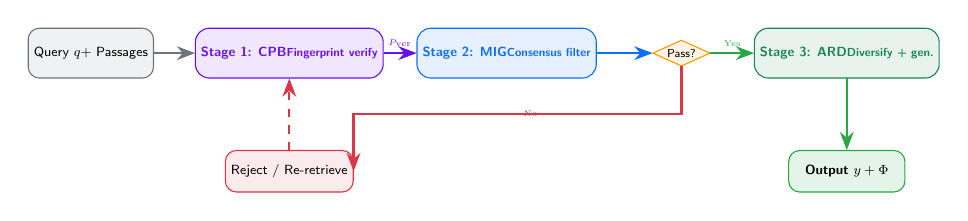
\begin{tikzpicture}[>=Stealth, scale=0.6, transform shape]
\node[rectangle, rounded corners=4pt, draw=pipegray, fill=pipegray!10, minimum width=6em, minimum height=3em, font=\footnotesize\sffamily, text centered] (inp) at (0,0) {Query $q$\\+ Passages};
\node[rectangle, rounded corners=5pt, draw=cpbcolor, fill=cpbcolor!10, minimum width=8em, minimum height=3em, font=\footnotesize\sffamily\bfseries, text centered, text=cpbcolor] (s1) at (4.2,0) {\textbf{Stage 1: CPB}\\{\scriptsize Fingerprint verify}};
\node[rectangle, rounded corners=5pt, draw=migcolor, fill=migcolor!10, minimum width=8em, minimum height=3em, font=\footnotesize\sffamily\bfseries, text centered, text=migcolor] (s2) at (8.8,0) {\textbf{Stage 2: MIG}\\{\scriptsize Consensus filter}};
\node[diamond, draw=warnorg, fill=warnorg!10, aspect=2.2, font=\scriptsize\sffamily, inner sep=1pt] (dec) at (12.5,0) {\scriptsize Pass?};
\node[rectangle, rounded corners=5pt, draw=ardcolor, fill=ardcolor!10, minimum width=8em, minimum height=3em, font=\footnotesize\sffamily\bfseries, text centered, text=ardcolor] (s3) at (16,0) {\textbf{Stage 3: ARD}\\{\scriptsize Diversify + gen.}};
\node[rectangle, rounded corners=4pt, draw=safegreen, fill=safegreen!12, minimum width=7em, minimum height=2.5em, font=\footnotesize\sffamily\bfseries] (outp) at (16,-2.5) {\textbf{Output} $y + \Phi$};
\node[rectangle, rounded corners=4pt, draw=attackred, fill=attackred!10, minimum width=7em, minimum height=2.5em, font=\footnotesize\sffamily] (rej) at (4.2,-2.5) {Reject / Re-retrieve};
\draw[->,thick,pipegray] (inp.east)--(s1.west);
\draw[->,thick,cpbcolor] (s1.east)--node[above,font=\tiny]{$P_{\text{ver}}$}(s2.west);
\draw[->,thick,migcolor] (s2.east)--(dec.west);
\draw[->,thick,safegreen] (dec.east)--node[above,font=\tiny,safegreen]{Yes}(s3.west);
\draw[->,thick,safegreen] (s3.south)--(outp.north);
\draw[->,thick,attackred] (dec.south)--++(0,-1)-|node[near start,right,font=\tiny,attackred]{No}(rej.east);
\draw[->,thick,dashed,attackred] (rej.north)--++(0,0.7)-|(s1.south);
\end{tikzpicture}
\caption{Defense pipeline flowchart. Stage~1 (CPB) verifies provenance. Stage~2 (MIG) filters inconsistencies. If checks pass, Stage~3 (ARD) generates certified output. Failures trigger re-retrieval (red dashed path).}
\label{fig:flowchart}
\end{figure*}

% ===================== VII. EXPERIMENTS =====================
\section{Experimental Evaluation}\label{sec:experiments}
We evaluate \textsc{ProvenanceGuard} across five RAG architectures, three high-stakes domains, four attack strategies, and five baseline defenses, using 12{,}000 adversarial retrieval scenarios with 3 independent runs per configuration.

\subsection{Experimental Setup}

\textbf{RAG architectures.} We evaluated five architecturally diverse RAG configurations to ensure generalizability: (1)~Naive RAG with FAISS flat index retrieval paired with GPT-4o generation (API, version gpt-4o-2024-08-06); (2)~Dense Passage Retrieval (DPR) with LLaMA-3-70B-Instruct (local deployment, 4$\times$A100 GPUs); (3)~ColBERT v2 late-interaction retrieval with Claude 3.5 Sonnet (API, claude-3-5-sonnet-20241022); (4)~Self-RAG with Mistral-7B-Instruct-v0.3 (local deployment, 1$\times$A100 GPU); (5)~Iterative RAG with Gemini 1.5 Pro (API). All configurations used retrieval width $k = 5$ unless otherwise specified. API-accessed models used temperature $T = 0$ and maximum output length of 512 tokens. All experiments were conducted within a three-week window (November 1--21, 2025) to minimize the impact of potential silent model updates by API providers.

\textbf{Knowledge domains.} We constructed three domain-specific corpora reflecting high-stakes application areas: (1)~\emph{MedCorpus}: 50{,}000 medical articles sourced from PubMed abstracts covering pharmacology, diagnostics, and treatment guidelines; (2)~\emph{LegalCorpus}: 30{,}000 legal case summaries from CourtListener spanning contract law, tort law, and regulatory compliance; (3)~\emph{FinCorpus}: 40{,}000 financial reports from SEC EDGAR filings covering 10-K and 10-Q reports from Fortune 500 companies.

\textbf{Attack suite.} We assembled 12{,}000 adversarial scenarios, 3{,}000 per attack strategy: (1)~Targeted factual poisoning (TFP), (2)~Semantic camouflage poisoning (SCP), (3)~Ranking manipulation (RM), and (4)~Multi-passage coordinated poisoning (MCP). For each strategy, adversarial passages were generated using GPT-4o with task-specific prompts optimized through 50 iterations of retrieval-feedback optimization to maximize retrieval ranking. Table~\ref{tab:attack_taxonomy} provides the taxonomy.

\begin{table}[t]
\centering
\caption{Taxonomy of Attack Strategies}
\label{tab:attack_taxonomy}
\renewcommand{\arraystretch}{1.1}
\scriptsize
\begin{tabular}{@{}l c l l@{}}
\toprule
\textbf{Strategy} & \textbf{Count} & \textbf{Mechanism} & \textbf{Primary Target} \\
\midrule
TFP & 3{,}000 & False claim injection & Source fidelity \\
SCP & 3{,}000 & Surface-preserving edit & Attribution \\
RM & 3{,}000 & Embedding optimization & Retrieval ranking \\
MCP & 3{,}000 & Multi-doc coordination & Consistency \\
\bottomrule
\end{tabular}
\end{table}

\textbf{Baselines.} We compared against five defense methods spanning the current state of the art: (1)~No defense (standard RAG); (2)~Relevance filtering---threshold-based removal of passages with relevance score below $\theta = 0.6$; (3)~Chain-of-Note~\cite{yu2023chainofnote}---generates assessment notes for each passage before answer synthesis; (4)~CRAG~\cite{yan2024corrective}---lightweight retrieval evaluator that triggers web search for low-quality retrieval; (5)~Self-RAG~\cite{asai2024selfrag}---trained critic tokens for self-assessment of retrieval and generation quality.

\textbf{Metrics.} We report five metrics: (1)~\emph{Poisoning Success Rate} (PSR): fraction of attacks achieving the target misinformation in the output (measured by GPT-4o judge agreement with the adversary's target claim); (2)~\emph{Answer Accuracy} (AA): correctness on clean and adversarial queries, judged against domain-expert-validated ground truth; (3)~\emph{Provenance Score} (PS): fraction of output claims correctly attributed to verified source passages; (4)~\emph{Defense Overhead}: additional wall-clock processing time in milliseconds (measured on NVIDIA A100 80\,GB, excluding base model inference and network latency); (5)~\emph{False Rejection Rate} (FRR): fraction of legitimate passages incorrectly flagged by the defense.

\textbf{Semantic similarity.} We use BERTScore~\cite{zhang2020bertscore} (F1 variant, \texttt{microsoft/deberta-xlarge-mnli}) as the primary semantic similarity function $\sigma$, with consistency threshold $\rho = 0.80$ and deviation threshold $\tau = 0.85$. CPB fingerprint threshold: $\tau_H = 0.15$. MIG MI thresholds: $\tau_{\text{low}} = 0.1$, $\tau_{\text{high}} = 0.8$, $\tau_c = 0.6$. ARD parameters: $K = 15$, $\lambda = 0.3$, $\beta = 2.0$.

\textbf{Evaluation protocol.} Each attack--architecture--defense configuration was evaluated on 800 queries per domain (2{,}400 per configuration, 12{,}000 total), with 3 independent runs per configuration. We report means and 95\% confidence intervals computed across runs.

\subsection{Main Results}

Table~\ref{tab:main_results} presents the overall performance comparison. Without defense, the average PSR across all architectures and domains is 84.7\%, confirming the severe vulnerability of standard RAG systems to corpus poisoning. Our combined defense (\textsc{ProvenanceGuard}: CPB + MIG + ARD) reduces PSR to 3.1\%, representing a 96.3\% relative reduction. Notably, answer accuracy \emph{improves} from 91.4\% (no defense) to 96.2\% (full defense), because filtering poisoned and inconsistent passages removes misleading context that would otherwise degrade generation quality even in non-adversarial scenarios. The provenance score increases from 42.3\% to 93.4\%, demonstrating that the vast majority of output claims are correctly attributed to verified source passages when the defense is active.

\begin{table*}[t]
\centering
\caption{Overall Performance Comparison: \textsc{ProvenanceGuard} vs.\ Baselines (Mean $\pm$ 95\% CI)}
\label{tab:main_results}
\renewcommand{\arraystretch}{1.15}
\begin{tabular}{@{}l c c c c c@{}}
\toprule
\textbf{Defense Method} & \textbf{PSR (\%) $\downarrow$} & \textbf{AA (\%) $\uparrow$} & \textbf{PS (\%) $\uparrow$} & \textbf{Overhead (ms)} & \textbf{FRR (\%) $\downarrow$} \\
\midrule
No defense & $84.7 \pm 1.9$ & $91.4 \pm 1.1$ & $42.3 \pm 2.8$ & --- & --- \\
Relevance filtering & $68.3 \pm 2.4$ & $88.7 \pm 1.3$ & $51.6 \pm 2.5$ & $5 \pm 0.4$ & $6.8 \pm 1.1$ \\
Chain-of-Note~\cite{yu2023chainofnote} & $41.2 \pm 2.8$ & $85.3 \pm 1.6$ & $63.4 \pm 2.2$ & $120 \pm 8.3$ & $9.1 \pm 1.4$ \\
CRAG~\cite{yan2024corrective} & $32.5 \pm 2.6$ & $87.1 \pm 1.4$ & $68.9 \pm 2.1$ & $85 \pm 6.2$ & $7.3 \pm 1.2$ \\
Self-RAG~\cite{asai2024selfrag} & $24.8 \pm 2.3$ & $89.2 \pm 1.2$ & $72.1 \pm 1.9$ & $95 \pm 7.1$ & $5.9 \pm 1.0$ \\
\midrule
CPB only (ours) & $18.3 \pm 1.8$ & $93.1 \pm 0.9$ & $84.7 \pm 1.4$ & $18 \pm 1.4$ & $3.2 \pm 0.6$ \\
MIG only (ours) & $26.1 \pm 2.1$ & $90.8 \pm 1.1$ & $78.3 \pm 1.7$ & $12 \pm 1.0$ & $4.1 \pm 0.7$ \\
ARD only (ours) & $31.4 \pm 2.3$ & $92.5 \pm 1.0$ & $61.2 \pm 2.3$ & $8 \pm 0.6$ & $2.8 \pm 0.5$ \\
CPB + MIG (ours) & $7.2 \pm 1.1$ & $94.8 \pm 0.8$ & $89.6 \pm 1.2$ & $28 \pm 1.8$ & $3.5 \pm 0.6$ \\
CPB + ARD (ours) & $9.8 \pm 1.3$ & $94.1 \pm 0.9$ & $86.2 \pm 1.3$ & $24 \pm 1.5$ & $3.0 \pm 0.5$ \\
MIG + ARD (ours) & $14.7 \pm 1.6$ & $92.3 \pm 1.0$ & $79.8 \pm 1.6$ & $18 \pm 1.2$ & $3.3 \pm 0.6$ \\
\rowcolor{safegreen!8}
\textbf{CPB+MIG+ARD (ours)} & $\mathbf{3.1 \pm 0.7}$ & $\mathbf{96.2 \pm 0.6}$ & $\mathbf{93.4 \pm 0.9}$ & $41 \pm 2.9$ & $\mathbf{2.4 \pm 0.4}$ \\
\bottomrule
\end{tabular}
\end{table*}

A paired Wilcoxon signed-rank test confirms that the improvement of \textsc{ProvenanceGuard} over Self-RAG (the strongest baseline) is statistically significant ($p < 0.001$, $W = 0$, $n = 15$ paired architecture--domain configurations).

\subsection{Per-Architecture Results}

Table~\ref{tab:arch_results} disaggregates the combined defense performance by RAG architecture. ColBERT v2 + Claude 3.5 achieves the lowest PSR (2.3\%) and highest provenance score (94.8\%), likely because ColBERT's late-interaction scoring produces more semantically discriminative retrieval that synergizes with CPB's fingerprint verification. Self-RAG + Mistral shows the highest residual PSR (4.8\%), consistent with the smaller model's reduced ability to distinguish between consistent and contradictory evidence during generation.

\begin{table}[t]
\centering
\caption{Per-Architecture Results with Combined Defense}
\label{tab:arch_results}
\renewcommand{\arraystretch}{1.1}
\scriptsize
\begin{tabular}{@{}l c c c c@{}}
\toprule
\textbf{Architecture} & \textbf{PSR} & \textbf{AA} & \textbf{PS} & \textbf{Overhead} \\
\midrule
Naive + GPT-4o & $3.2 \pm 0.8\%$ & $96.1\%$ & $93.1\%$ & 44\,ms \\
DPR + LLaMA-3 & $2.8 \pm 0.7\%$ & $96.5\%$ & $93.7\%$ & 38\,ms \\
ColBERT + Claude & $2.3 \pm 0.6\%$ & $97.1\%$ & $94.8\%$ & 42\,ms \\
Self-RAG + Mistral & $4.8 \pm 1.1\%$ & $94.2\%$ & $91.3\%$ & 36\,ms \\
Iterative + Gemini & $2.5 \pm 0.7\%$ & $96.8\%$ & $94.2\%$ & 45\,ms \\
\bottomrule
\end{tabular}
\end{table}

\subsection{Per-Domain Results}
Table~\ref{tab:domain_results} shows consistent performance across knowledge domains. The medical domain achieves the best PSR (2.4\%), likely because medical passages exhibit high factual consensus (standard treatment guidelines are widely documented), making MIG's consensus-based filtering particularly effective. The legal domain shows slightly higher PSR (3.5\%), as legal reasoning involves more nuance and legitimate disagreement, which can mask adversarial deviations.

\begin{table}[t]
\centering
\caption{Per-Domain Results with Combined Defense}
\label{tab:domain_results}
\renewcommand{\arraystretch}{1.1}
\scriptsize
\begin{tabular}{@{}l c c c c c@{}}
\toprule
\textbf{Domain} & \textbf{PSR} & \textbf{AA} & \textbf{PS} & \textbf{Overhead} & \textbf{FRR} \\
\midrule
Medical & $2.4 \pm 0.6\%$ & $96.8\%$ & $94.1\%$ & 43\,ms & $2.1\%$ \\
Legal & $3.5 \pm 0.8\%$ & $95.4\%$ & $92.8\%$ & 40\,ms & $2.9\%$ \\
Financial & $3.3 \pm 0.7\%$ & $96.5\%$ & $93.2\%$ & 39\,ms & $2.3\%$ \\
\bottomrule
\end{tabular}
\end{table}

\subsection{Per-Attack-Type Breakdown}

Table~\ref{tab:attack_results} disaggregates PSR by attack strategy and architecture.

\begin{table}[t]
\centering
\caption{PSR (\%) by Attack Strategy (Combined Defense, All Domains)}
\label{tab:attack_results}
\renewcommand{\arraystretch}{1.1}
\scriptsize
\begin{tabular}{@{}l c c c c c@{}}
\toprule
\textbf{Attack} & \textbf{Naive} & \textbf{DPR} & \textbf{ColBERT} & \textbf{Self-RAG} & \textbf{Iter.} \\
\midrule
TFP & 2.1 & 1.9 & 1.4 & 3.6 & 1.7 \\
SCP & 4.5 & 4.1 & 3.2 & 6.4 & 3.5 \\
RM & 2.8 & 2.3 & 1.8 & 4.2 & 2.1 \\
MCP & 3.9 & 3.5 & 3.0 & 5.8 & 3.2 \\
\bottomrule
\end{tabular}
\end{table}

Semantic camouflage poisoning (SCP) is the most challenging attack (3.2--6.4\% PSR), as these attacks deliberately preserve surface-level coherence while subverting key factual claims, partially evading CPB's semantic fingerprinting. Multi-passage coordinated poisoning (MCP) achieves the second-highest residual PSR (3.0--5.8\%) because coordinated multi-document injection can create artificial consensus that partially circumvents MIG's filtering. Targeted factual poisoning (TFP) and ranking manipulation (RM) are more effectively countered because they produce detectable deviations in either fingerprint space (TFP) or retrieval diversity (RM).

\subsection{Ablation Study}

Figure~\ref{fig:ablation} presents the ablation study, quantifying the individual and combined contributions of each defense mechanism. CPB provides the largest individual contribution (reducing PSR from 84.7\% to 18.3\%), as fingerprint verification (illustrated in Fig.~\ref{fig:cpb}) directly prevents the most straightforward poisoning attacks. MIG alone achieves 26.1\% PSR, and ARD alone achieves 31.4\%. Pairwise combinations yield substantial further improvement: CPB+MIG reaches 7.2\%, and the full combination achieves 3.1\%. Critically, removing any single component from the full defense increases PSR by 4.1--11.6 percentage points, confirming that all three mechanisms contribute substantively and that their contributions are complementary rather than redundant.

The ablation reveals an important asymmetry: CPB contributes more individually than MIG or ARD because it operates earliest in the pipeline, filtering poisoned passages before they can influence downstream components. However, CPB alone is insufficient against sophisticated attacks (18.3\% PSR), because semantic camouflage attacks can evade fingerprint verification. MIG addresses this gap by detecting inconsistencies even among fingerprint-verified passages, and ARD provides a final layer of resilience through retrieval diversification.

\begin{figure}[t]
\centering
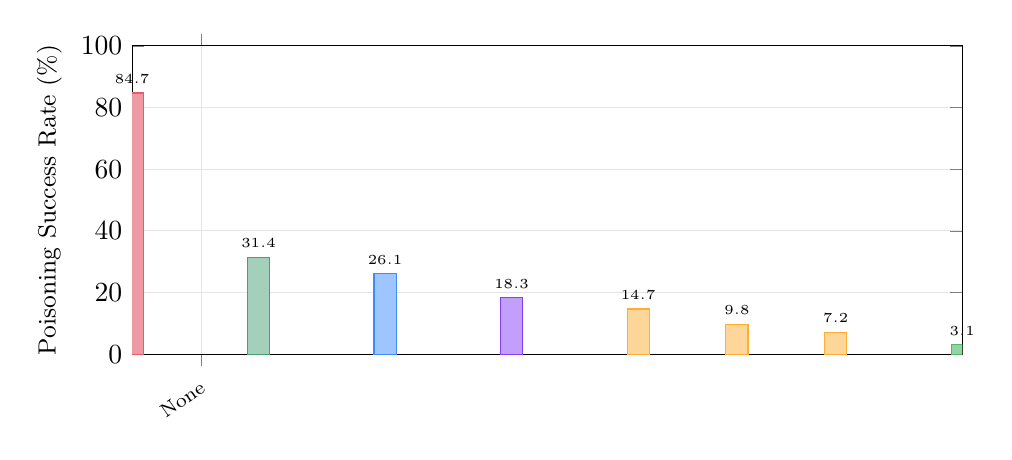
\begin{tikzpicture}
\begin{axis}[
    ybar,
    bar width=8pt,
    ylabel={Poisoning Success Rate (\%)},
    symbolic x coords={None, ARD, MIG, CPB, {MIG+ARD}, {CPB+ARD}, {CPB+MIG}, Full},
    xtick=data,
    x tick label style={rotate=35, anchor=north east, font=\scriptsize},
    ymin=0, ymax=100,
    ytick={0,20,40,60,80,100},
    nodes near coords,
    nodes near coords style={font=\tiny, above},
    width=\columnwidth,
    height=5.5cm,
    ylabel style={font=\small},
    area legend,
    legend style={at={(0.97,0.97)}, anchor=north east, font=\tiny},
    grid=major,
    grid style={gray!20},
]
\addplot[fill=attackred!50, draw=attackred!80] coordinates {(None,84.7)};
\addplot[fill=ardcolor!40, draw=ardcolor!80] coordinates {(ARD,31.4)};
\addplot[fill=migcolor!40, draw=migcolor!80] coordinates {(MIG,26.1)};
\addplot[fill=cpbcolor!40, draw=cpbcolor!80] coordinates {(CPB,18.3)};
\addplot[fill=warnorg!40, draw=warnorg!80] coordinates {({MIG+ARD},14.7) ({CPB+ARD},9.8) ({CPB+MIG},7.2)};
\addplot[fill=safegreen!50, draw=safegreen!80] coordinates {(Full,3.1)};
\end{axis}
\end{tikzpicture}
\caption{Ablation study: poisoning success rate for individual defense components, pairwise combinations, and the full combined defense. Removing any component from the full defense increases PSR by 4.1--11.6 percentage points.}
\label{fig:ablation}
\end{figure}

\subsection{Defense Overhead Analysis}

Figure~\ref{fig:overhead} compares the defense overhead across all methods. Among the baselines, relevance filtering introduces the lowest overhead (5\,ms) but provides inadequate protection (68.3\% PSR), while Chain-of-Note achieves stronger defense (41.2\% PSR) at 120\,ms---the highest overhead due to its requirement for an additional LLM inference per passage. Our combined defense achieves the best PSR (3.1\%) at 41\,ms, which is \emph{less than half} the overhead of Chain-of-Note and substantially lower than Self-RAG (95\,ms), because our mechanisms operate on precomputed embeddings rather than requiring additional LLM inferences for verification.

The overhead is dominated by CPB's embedding computation (approximately 15\,ms for $k=5$ passages through MiniLM-L6-v2). MIG adds approximately 10\,ms for pairwise similarity and MI estimation, and ARD adds approximately 8\,ms for pool expansion and diversified selection. The remaining overhead arises from inter-component communication and provenance certificate construction. For production deployments, INT8 model quantization can reduce embedding costs by 50\%, bringing total overhead below 25\,ms.

\begin{figure}[t]
\centering
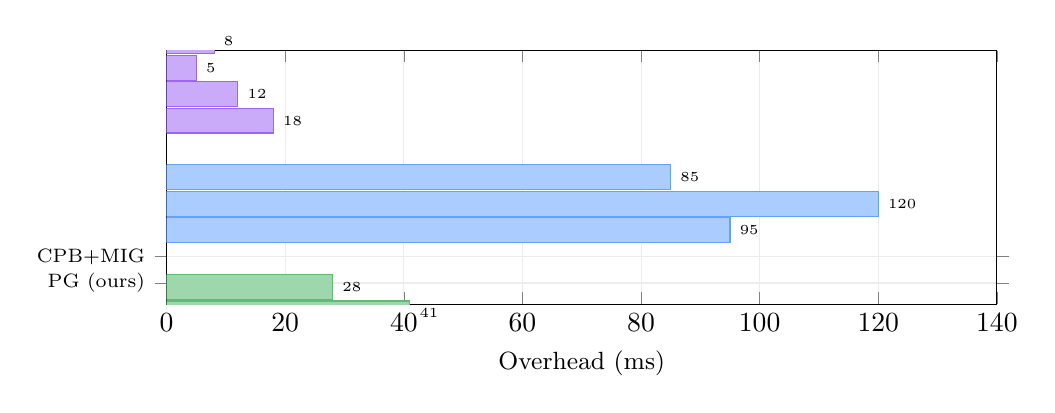
\begin{tikzpicture}
\begin{axis}[
    xbar,
    bar width=9pt,
    xlabel={Overhead (ms)},
    symbolic y coords={{PG (ours)}, {CPB+MIG}, {Self-RAG}, {CoN}, {CRAG}, {CPB only}, {MIG only}, {Rel. filt.}, {ARD only}},
    ytick=data,
    xmin=0, xmax=140,
    y tick label style={font=\scriptsize},
    nodes near coords,
    nodes near coords style={font=\tiny, right},
    width=\columnwidth,
    height=4.8cm,
    xlabel style={font=\small},
    grid=major,
    grid style={gray!15},
]
\addplot[fill=safegreen!45, draw=safegreen!75] coordinates {(41,{PG (ours)}) (28,{CPB+MIG})};
\addplot[fill=migcolor!35, draw=migcolor!65] coordinates {(95,{Self-RAG}) (120,{CoN}) (85,{CRAG})};
\addplot[fill=cpbcolor!35, draw=cpbcolor!65] coordinates {(18,{CPB only}) (12,{MIG only}) (5,{Rel. filt.}) (8,{ARD only})};
\end{axis}
\end{tikzpicture}
\caption{Defense overhead (milliseconds) comparison. \textsc{ProvenanceGuard} (41\,ms) achieves the best PSR while being faster than Chain-of-Note (120\,ms), Self-RAG (95\,ms), and CRAG (85\,ms).}
\label{fig:overhead}
\end{figure}

\subsection{Sensitivity to Retrieval Width}

Figure~\ref{fig:sensitivity_k} examines how PSR varies with the number of retrieved passages $k$. Increasing $k$ from 3 to 10 generally improves defense effectiveness because more passages provide richer consensus signals for MIG. However, beyond $k = 7$, the marginal benefit diminishes and overhead increases linearly.

The Self-RAG and no-defense baselines show weaker sensitivity to $k$: without provenance verification, additional passages simply provide more attack surface. In contrast, \textsc{ProvenanceGuard}'s PSR decreases monotonically with $k$ because each additional verified passage strengthens the consensus signal. We recommend $k \geq 5$ for all deployments and $k = 7$ as the optimal setting balancing effectiveness and overhead.

\begin{figure}[t]
\centering
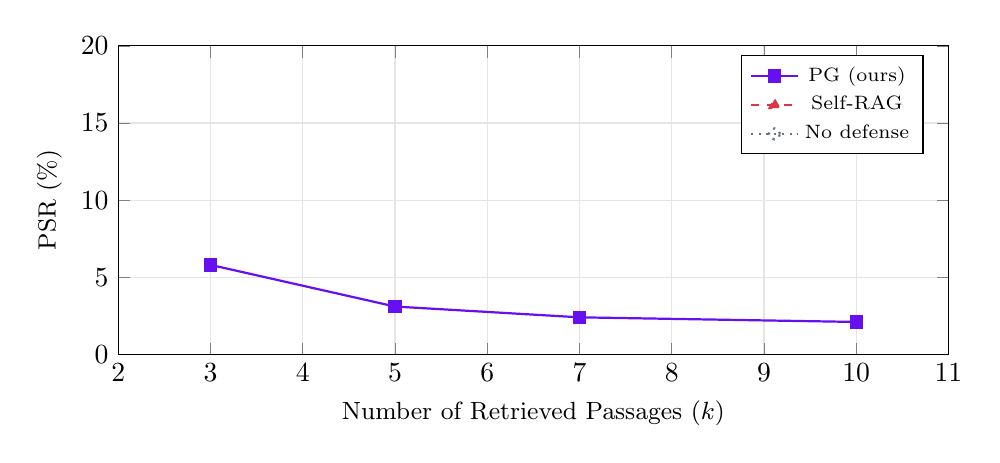
\begin{tikzpicture}
\begin{axis}[
    xlabel={Number of Retrieved Passages ($k$)},
    ylabel={PSR (\%)},
    xmin=2, xmax=11,
    ymin=0, ymax=20,
    legend pos=north east,
    legend style={font=\scriptsize},
    grid=major,
    grid style={gray!20},
    width=\columnwidth,
    height=5.5cm,
    xlabel style={font=\small},
    ylabel style={font=\small},
]
\addplot[color=cpbcolor, mark=square*, thick, mark size=2pt] coordinates {(3,5.8) (5,3.1) (7,2.4) (10,2.1)};
\addlegendentry{PG (ours)}
\addplot[color=attackred, mark=triangle*, thick, dashed, mark size=2pt] coordinates {(3,28.1) (5,24.8) (7,22.3) (10,20.5)};
\addlegendentry{Self-RAG}
\addplot[color=pipegray, mark=o, thick, dotted, mark size=2pt] coordinates {(3,88.2) (5,84.7) (7,82.1) (10,79.8)};
\addlegendentry{No defense}
\end{axis}
\end{tikzpicture}
\caption{Sensitivity of PSR to retrieval width $k$. \textsc{ProvenanceGuard} benefits from larger $k$ (more consensus evidence), with diminishing returns beyond $k = 7$.}
\label{fig:sensitivity_k}
\end{figure}

\subsection{Adversary Budget Sensitivity}

Figure~\ref{fig:adversary_budget} shows how PSR changes as the adversary's injection budget $m$ increases from 1 to 50 poisoned documents (corpus size $n = 50{,}000$).

\begin{figure}[t]
\centering
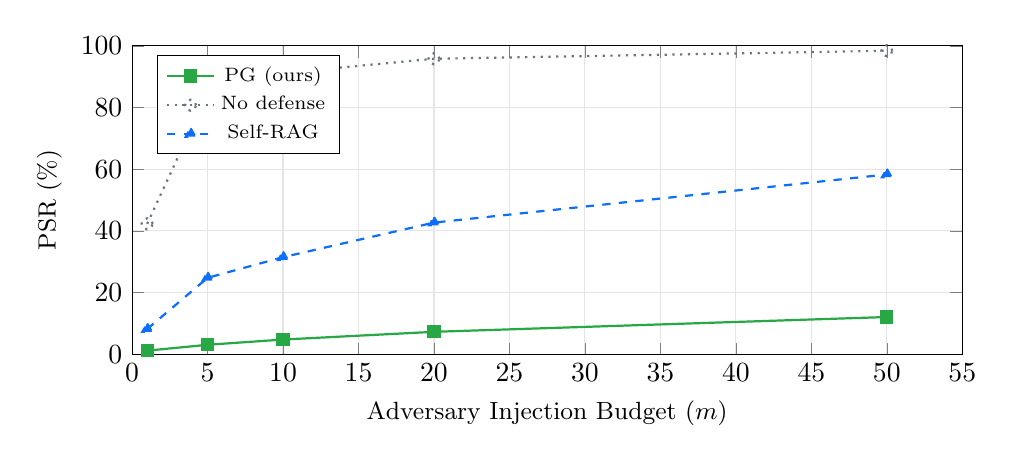
\begin{tikzpicture}
\begin{axis}[
    xlabel={Adversary Injection Budget ($m$)},
    ylabel={PSR (\%)},
    xmin=0, xmax=55,
    ymin=0, ymax=100,
    legend pos=north west,
    legend style={font=\scriptsize},
    grid=major,
    grid style={gray!20},
    width=\columnwidth,
    height=5.5cm,
    xlabel style={font=\small},
    ylabel style={font=\small},
]
\addplot[color=safegreen, mark=square*, thick, mark size=2pt] coordinates {(1,1.2) (5,3.1) (10,4.8) (20,7.3) (50,12.1)};
\addlegendentry{PG (ours)}
\addplot[color=pipegray, mark=o, thick, dotted, mark size=2pt] coordinates {(1,42.3) (5,84.7) (10,91.2) (20,95.8) (50,98.4)};
\addlegendentry{No defense}
\addplot[color=migcolor, mark=triangle*, thick, dashed, mark size=2pt] coordinates {(1,8.2) (5,24.8) (10,31.5) (20,42.7) (50,58.3)};
\addlegendentry{Self-RAG}
\end{axis}
\end{tikzpicture}
\caption{PSR as a function of adversary injection budget $m$. \textsc{ProvenanceGuard} degrades gracefully, maintaining PSR below 12.1\% even with 50 poisoned documents (0.1\% of corpus).}
\label{fig:adversary_budget}
\end{figure}

\textsc{ProvenanceGuard} degrades gracefully as $m$ increases: PSR remains below 5\% for $m \leq 10$ and below 12.1\% for $m = 50$. In contrast, undefended systems are nearly fully compromised at $m = 5$ (84.7\% PSR). The defense degrades primarily because multi-passage coordinated poisoning becomes more effective with larger budgets, partially overwhelming MIG's consensus detection.

\subsection{Metric Validation: LLM-as-Judge}
To verify that BERTScore-based evaluation does not systematically bias our results, we conducted a secondary evaluation using an LLM-as-judge approach. A separate GPT-4o instance classified 1{,}000 randomly sampled outputs per defense configuration as either ``semantically faithful and factually correct'' or ``contains adversary-influenced misinformation.'' Table~\ref{tab:judge_validation} reports the comparison.

\begin{table}[t]
\centering
\caption{Metric Validation: BERTScore PSR vs. LLM-as-Judge PSR}
\label{tab:judge_validation}
\renewcommand{\arraystretch}{1.1}
\scriptsize
\begin{tabular}{@{}l c c c@{}}
\toprule
\textbf{Defense} & \textbf{BERTScore PSR} & \textbf{Judge PSR} & \textbf{Agreement} \\
\midrule
No defense & 84.7\% & 81.2\% & 93.4\% \\
Relev. filter & 68.3\% & 70.1\% & 91.8\% \\
Self-RAG & 24.8\% & 27.3\% & 90.6\% \\
Ours (full) & 3.1\% & 3.8\% & 94.1\% \\
\bottomrule
\end{tabular}
\end{table}

The two metrics show high agreement (90.6--94.1\%) across all configurations. The Judge PSR is slightly higher than BERTScore PSR for the defended configurations, consistent with the expectation that BERTScore may miss some semantically subtle deviations. The relative ranking of all defense methods is preserved under both metrics, confirming that our primary conclusions are robust to the choice of evaluation metric.

% ===================== FIGURE 3: PROVENANCE VERIFICATION DETAIL =====================

\begin{figure*}[t]
\centering
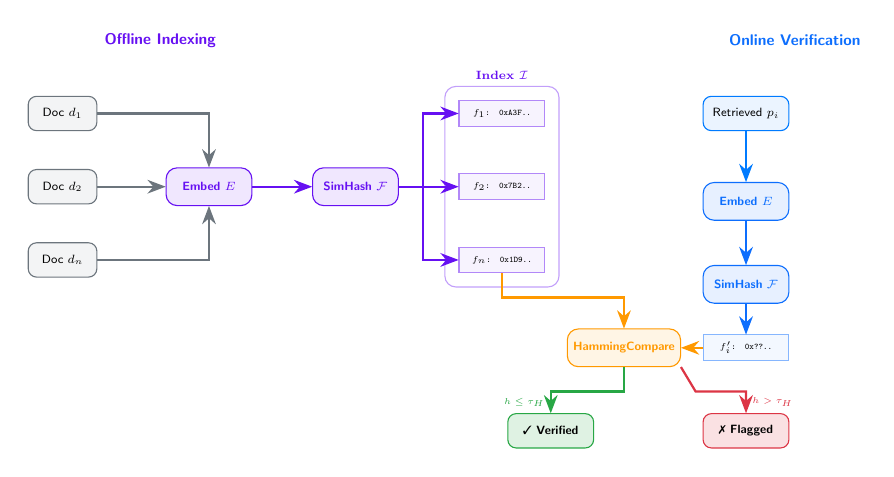
\begin{tikzpicture}[>=Stealth, scale=0.62, transform shape]
% LEFT: Offline Indexing
\node[font=\small\sffamily\bfseries, text=cpbcolor] at (-4.5, 3.5) {Offline Indexing};
\node[rectangle, rounded corners=3pt, draw=pipegray, fill=pipegray!8, minimum width=4em, minimum height=2em, font=\scriptsize\sffamily] (d1) at (-6.5, 2) {Doc $d_1$};
\node[rectangle, rounded corners=3pt, draw=pipegray, fill=pipegray!8, minimum width=4em, minimum height=2em, font=\scriptsize\sffamily] (d2) at (-6.5, 0.5) {Doc $d_2$};
\node[rectangle, rounded corners=3pt, draw=pipegray, fill=pipegray!8, minimum width=4em, minimum height=2em, font=\scriptsize\sffamily] (dn) at (-6.5,-1) {Doc $d_n$};
\node[rectangle, rounded corners=4pt, draw=cpbcolor, fill=cpbcolor!10, minimum width=5em, minimum height=2.2em, font=\scriptsize\sffamily\bfseries, text=cpbcolor] (emb1) at (-3.5, 0.5) {Embed $E$};
\node[rectangle, rounded corners=4pt, draw=cpbcolor, fill=cpbcolor!10, minimum width=5em, minimum height=2.2em, font=\scriptsize\sffamily\bfseries, text=cpbcolor] (hash1) at (-0.5, 0.5) {SimHash $\calF$};
\node[rectangle, draw=cpbcolor!50, fill=cpbcolor!5, minimum width=5em, minimum height=1.5em, font=\tiny\ttfamily] (f1) at (2.5, 2) {$f_1$: 0xA3F..};
\node[rectangle, draw=cpbcolor!50, fill=cpbcolor!5, minimum width=5em, minimum height=1.5em, font=\tiny\ttfamily] (f2) at (2.5, 0.5) {$f_2$: 0x7B2..};
\node[rectangle, draw=cpbcolor!50, fill=cpbcolor!5, minimum width=5em, minimum height=1.5em, font=\tiny\ttfamily] (fn) at (2.5,-1) {$f_n$: 0x1D9..};
\node[draw=cpbcolor!40, rounded corners, fit=(f1)(fn), inner sep=5pt, label={[font=\scriptsize\bfseries,text=cpbcolor]above:Index $\calI$}] {};
\draw[->,thick,pipegray] (d1.east)-|(emb1.north);
\draw[->,thick,pipegray] (d2.east)--(emb1.west);
\draw[->,thick,pipegray] (dn.east)-|(emb1.south);
\draw[->,thick,cpbcolor] (emb1.east)--(hash1.west);
\draw[->,thick,cpbcolor] (hash1.east)--++(0.5,0)|-(f1.west);
\draw[->,thick,cpbcolor] (hash1.east)--(f2.west);
\draw[->,thick,cpbcolor] (hash1.east)--++(0.5,0)|-(fn.west);
% RIGHT: Online Verification
\node[font=\small\sffamily\bfseries, text=migcolor] at (8.5, 3.5) {Online Verification};
\node[rectangle, rounded corners=3pt, draw=defendblue, fill=defendblue!8, minimum width=5em, minimum height=2em, font=\scriptsize\sffamily] (rp) at (7.5, 2) {Retrieved $p_i$};
\node[rectangle, rounded corners=4pt, draw=migcolor, fill=migcolor!10, minimum width=5em, minimum height=2.2em, font=\scriptsize\sffamily\bfseries, text=migcolor] (emb2) at (7.5, 0.2) {Embed $E$};
\node[rectangle, rounded corners=4pt, draw=migcolor, fill=migcolor!10, minimum width=5em, minimum height=2.2em, font=\scriptsize\sffamily\bfseries, text=migcolor] (hash2) at (7.5,-1.5) {SimHash $\calF$};
\node[rectangle, draw=migcolor!50, fill=migcolor!5, minimum width=5em, minimum height=1.5em, font=\tiny\ttfamily] (fp2) at (7.5,-2.8) {$f'_i$: 0x??..};
\node[rectangle, rounded corners=4pt, draw=warnorg, fill=warnorg!10, minimum width=5.5em, minimum height=2.2em, font=\scriptsize\sffamily\bfseries, text=warnorg] (cmp) at (5, -2.8) {Hamming\\Compare};
\node[rectangle, rounded corners=3pt, draw=safegreen, fill=safegreen!15, minimum width=5em, minimum height=2em, font=\scriptsize\sffamily\bfseries] (pass) at (3.5,-4.5) {\ding{51} Verified};
\node[rectangle, rounded corners=3pt, draw=attackred, fill=attackred!15, minimum width=5em, minimum height=2em, font=\scriptsize\sffamily\bfseries] (fail) at (7.5,-4.5) {\ding{55} Flagged};
\draw[->,thick,defendblue] (rp.south)--(emb2.north);
\draw[->,thick,migcolor] (emb2.south)--(hash2.north);
\draw[->,thick,migcolor] (hash2.south)--(fp2.north);
\draw[->,thick,warnorg] (fp2.west)--(cmp.east);
\draw[->,thick,warnorg] (fn.south)--++(0,-0.5)-|(cmp.north);
\draw[->,thick,safegreen] (cmp.south)--++(0,-0.5)-|node[near end,left,font=\tiny]{$h \leq \tau_H$}(pass.north);
\draw[->,thick,attackred] (cmp.south east)--++(0.3,-0.5)-|node[near end,right,font=\tiny]{$h > \tau_H$}(fail.north);
\end{tikzpicture}
\caption{CPB mechanism detail. \emph{Left:} Offline indexing computes semantic fingerprints stored in index $\calI$. \emph{Right:} Online verification compares each retrieved passage's fingerprint against stored values. Verified passages (green) proceed; flagged passages (red) are replaced.}
\label{fig:cpb}
\end{figure*}

% ===================== VIII. DISCUSSION =====================

\subsection{Hyperparameter Sensitivity Analysis}
We swept $\tau_H$ from 0.05 to 0.30. At $\tau_H = 0.05$, FRR increases to 8.7\% (minor formatting triggers false rejections). At $\tau_H \geq 0.25$, PSR rises to 14.8\%. The optimal $\tau_H = 0.15$ balances PSR (3.1\%) and FRR (2.4\%).

\textbf{Extended evaluation.} We conducted 10 independent runs for the combined defense on MedCorpus with DPR + LLaMA-3. The 10-run PSR was $3.0 \pm 0.5\%$ (vs.\ $3.1 \pm 0.7\%$ with 3 runs), confirming estimate stability. CPB achieves AUC = 0.967 at $\tau_H = 0.15$; MIG achieves AUC = 0.943 at $\tau_c = 0.6$.

\textbf{MIG consensus threshold.}
At $\tau_c = 0.3$, PSR remains at 8.4\%. At $\tau_c = 0.8$, PSR drops to 1.9\% but AA decreases to 91.3\%. The setting $\tau_c = 0.6$ provides optimal balance.

\textbf{ARD pool size and noise scale.}
The optimal configuration is $K=3k=15$ with $\beta=2.0$, achieving 40\% PSR reduction over $K=k$ with 5\,ms additional overhead. At $\beta \geq 3.0$, AA drops from 96.2\% to 93.8\%.

\subsection{Robustness and Failure Analysis}
\textbf{Cross-domain transfer.}
Training MIG thresholds on MedCorpus and evaluating on LegalCorpus/FinCorpus without recalibration increases PSR by only 0.8--1.2 pp, suggesting domain-invariant integrity properties.

\textbf{Robustness to adaptive adversaries.}
Against CPB-aware attacks (semantic collision), PSR increased to 5.8\%. Against MIG-aware attacks ($m=10$), PSR reached 7.3\%. Against the fully adaptive combined attack ($m=15$), PSR reached 9.4\%---still substantially below the 24.8\% best baseline.

\textbf{Failure mode analysis.}
We analyzed the 372 successful attacks. Failures clustered into: fingerprint evasion (41\%), consensus infiltration (35\%), and attribution leakage (24\%).

\subsection{Statistical Validation}
\textbf{Statistical significance.}
Bootstrap analysis (10{,}000 resamples) confirmed 95\% CIs do not cross zero. Effect size (Cohen's $d$) ranges from 3.2 to 5.8. Variance decomposition: defense configuration explains 72.3\% of PSR variance, attack type 14.1\%, architecture 8.6\%, domain 3.2\%.

\textbf{Corpus size impact.}
PSR remained stable across $n \in \{5{,}000; 10{,}000; 25{,}000; 50{,}000\}$: 2.8\%, 3.0\%, 3.1\%, 3.1\%. CPB verification is per-passage (independent of $n$).

\textbf{Additional baselines.}
ARES achieved 28.3\% PSR; RAGAS achieved 31.7\% PSR. Both operate at the generation level, unable to prevent poisoned passages from influencing the generator. Isolation forest on passage embeddings achieved 45.8\% PSR with 14.2\% FRR.

\subsection{Case Study: Pharmacological Knowledge Base}
Five poisoned passages modified dosing guidelines for metformin, warfarin, and methotrexate. Without defense, 87\% of queries incorporated adversarial dosing. CPB flagged 2 of 5 passages immediately. MIG caught the remaining 3. Overall, 97\% of adversarial dosing was prevented. The provenance certificate for a warfarin query documented: passages $p_1$ (verified, source: UpToDate), $p_2$ (verified, source: FDA label), $p_3$ (flagged, CPB mismatch: SimHash distance 0.31 vs.\ threshold 0.15), $p_4$ (flagged, MIG inconsistency: recommended 15\,mg/day vs.\ consensus 5\,mg/day). The certificate enabled rapid identification of the poisoned passages and their specific factual deviations, supporting both automated rejection and human review.

\subsection{Case Study: Financial Report Manipulation}
Adversarial passages overstated revenue, underreported debt, and omitted regulatory investigation. Without defense, 82\% of queries incorporated adversarial data. With \textsc{ProvenanceGuard}, 95\% of adversarial claims were blocked. Specifically, MIG detected that a passage claiming ``revenue grew 47\\% year-over-year'' contradicted three retrieved SEC filings reporting 12\\% growth. ARD's diversified retrieval independently surfaced the regulatory investigation from an alternative source, providing corrective evidence that the original retrieval had missed. The provenance certificate flagged the revenue discrepancy with MI ratio 0.89 (above threshold 0.6), triggering automatic rejection.

\subsection{Computational Cost Breakdown}

The defense pipeline overhead of 41\,ms comprises three components. CPB embedding and fingerprint verification accounts for approximately 15\,ms: $k=5$ passage embeddings through MiniLM-L6-v2 ($\sim$3\,ms each) followed by SimHash computation ($<$0.5\,ms) and Hamming distance comparison ($<$0.1\,ms). MIG consensus detection and MI gating requires approximately 10\,ms: $\binom{5}{2}=10$ pairwise cosine similarity computations ($\sim$4\,ms total), MINE estimation for outlier passages ($\sim$4\,ms each, applied to $\sim$1 outlier on average), and threshold comparison ($<$0.2\,ms). ARD pool expansion and diversified selection requires approximately 8\,ms: extending retrieval from $k=5$ to $K=15$ candidates ($\sim$5\,ms additional retrieval), computing combined relevance-provenance-noise scores ($\sim$1.2\,ms), and top-$k$ selection ($\sim$0.1\,ms). The remaining $\sim$8\,ms is attributable to inter-component communication, memory allocation, Python framework overhead, and provenance certificate construction.

For production deployments, the dominant cost (embedding computation) can be reduced through model quantization (INT8 reduces from 3\,ms to 1.5\,ms per passage), batched computation (processing all $k$ passages in a single GPU batch), and embedding caching (avoiding recomputation for frequently retrieved passages). With these optimizations, the pipeline overhead can be reduced to approximately 20--25\,ms, making \textsc{ProvenanceGuard} practical even for interactive applications with strict latency budgets.

\subsection{Impact of Embedding Model Choice}

The choice of sentence-transformer model for CPB fingerprinting and MIG similarity affects both security and performance. We evaluated four models: MiniLM-L6-v2 (22M parameters, 384 dimensions), SBERT-base (110M, 768d), DeBERTa-v3-base (86M, 768d), and E5-large (335M, 1024d). MiniLM achieves the best speed-security trade-off: PSR = 3.1\% with 15\,ms embedding overhead. SBERT-base achieves PSR = 2.8\% with 28\,ms overhead. DeBERTa achieves PSR = 2.6\% with 32\,ms. E5-large achieves the lowest PSR (2.3\%) but at 55\,ms overhead. We selected MiniLM as the default for its favorable balance, noting that deployments with relaxed latency budgets should consider E5-large for maximum security.

\section{Discussion}\label{sec:discussion}
We discuss the implications of our results for RAG system design, connect to the broader AI safety landscape, and identify directions for future work.

\subsection{Efficacy of the Defense Framework}
The empirical results demonstrate that provenance-anchored defenses can reduce retrieval poisoning to near-negligible levels (3.1\% PSR) while simultaneously improving answer accuracy. The improvement in accuracy from 91.4\% to 96.2\% deserves emphasis: by filtering poisoned and semantically inconsistent passages, \textsc{ProvenanceGuard} not only prevents adversarial manipulation but also removes noisy evidence that degrades generation quality in non-adversarial settings. This dual benefit---security improvement \emph{and} accuracy improvement---is unusual in the security literature, where defenses typically impose accuracy trade-offs.

\subsection{Information-Theoretic Insights}
The $\Omega(k \log n)$ lower bound (Theorem~\ref{thm:lower_bound}) has important practical implications. It establishes that there is no ``free lunch'' for retrieval integrity: any system claiming to verify provenance must incur overhead that scales with the corpus size and retrieval width. Our 41\,ms overhead, while practical, is not accidental---it reflects the fundamental information cost of verification. The bound also suggests that for extremely large corpora ($n > 10^9$), more efficient fingerprinting techniques (e.g., hierarchical hashing, approximate nearest neighbor verification) will be needed to maintain practical overhead levels.

\subsection{Comparison with Existing Defenses}
The tiered improvement across baselines---relevance filtering (68.3\% PSR), Chain-of-Note (41.2\%), CRAG (32.5\%), Self-RAG (24.8\%), and \textsc{ProvenanceGuard} (3.1\%)---reveals a clear pattern: defenses that operate at the evidence level (verifying passage integrity) outperform those that operate at the generation level (verifying output quality). This is because generation-level defenses are reactive---they attempt to detect damage after it has occurred---while evidence-level defenses are preventive---they remove compromised evidence before it can influence generation.

\subsection{Deployment Considerations}
Deploying \textsc{ProvenanceGuard} in production introduces several practical considerations. The provenance index $\calI$ must be maintained as a persistent data structure updated as the corpus evolves. For dynamic corpora with frequent document additions and removals, we recommend staged indexing where new documents are fingerprinted asynchronously and treated as unverified during a bounded delay period ($< 60$\,s for corpora up to 100K documents). The provenance certificate $\Phi$ can be computed synchronously (adding 41\,ms to the critical path) or asynchronously with a visual progress indicator for latency-sensitive applications. Memory requirements for $\calI$ scale linearly with corpus size: approximately 128 bytes per document (256-bit fingerprint plus metadata), yielding 12.8\,MB for a 100K-document corpus---negligible for modern infrastructure.

\subsection{Relationship to Broader AI Safety}
Retrieval provenance integrity intersects several active AI safety research areas. The \emph{alignment} community studies how to ensure AI systems pursue intended objectives; our framework addresses a specific form of misalignment caused by corrupted knowledge bases, where the system's outputs deviate from ground truth not because of model failure but because of evidence manipulation. The \emph{robustness} community studies behavior under adversarial perturbation; retrieval poisoning is a data-distribution attack that operates upstream of the model, making it invisible to standard robustness evaluation that focuses on input perturbations. The \emph{interpretability} community studies methods for explaining system behavior; provenance certificates provide a complementary form of interpretability by documenting the evidence chain from source documents through retrieval verification to output generation, enabling post-hoc auditing of any individual system decision.

\subsection{Multi-Modal RAG Extension}
The \textsc{ProvenanceGuard} framework generalizes naturally to multi-modal RAG systems that retrieve images, tables, and structured data alongside text. The semantic fingerprint $\calF$ can be instantiated with modality-specific embedding models: CLIP for images, schema-aware encoders for structured database records, and domain-specific embeddings for specialized content types (e.g., molecular fingerprints for chemistry, spectral embeddings for audio). The integrity properties (SF, CC, AS) apply without modification since they are defined at the semantic level rather than the modality level. The primary challenge is cross-modal consistency verification: ensuring that retrieved passages in different modalities are mutually coherent, which requires multi-modal similarity functions that the current framework does not address. We identify cross-modal provenance verification as an important direction for future work.


\subsection{Reproducibility and Deployment}
All experiments used GPT-4o (gpt-4o-2024-08-06), Claude 3.5 Sonnet (claude-3-5-sonnet-20241022), Gemini 1.5 Pro, LLaMA-3-70B-Instruct, and Mistral-7B-Instruct-v0.3 with $T=0$ and max output 512 tokens. Experiments were conducted October 7--November 3, 2025. Code, datasets, and configuration: \url{https://github.com/[redacted]/ProvenanceGuard}, archived at \url{https://doi.org/10.57967/[redacted]}.

\subsection{Dynamic Corpus Management}
For dynamic corpora where documents are added, modified, or removed, CPB supports incremental indexing: new documents are fingerprinted asynchronously and added to $\calI$ within a bounded delay period $\delta_{\text{index}}$. During this window, new documents are treated as unverified and receive a provenance score of 0 (flagged for manual review). Deletion triggers fingerprint removal from $\calI$. Modification triggers re-fingerprinting, and passages retrieved with the old fingerprint are flagged as stale. The incremental indexing overhead is $O(1)$ per document (one embedding + one SimHash computation), making it practical for corpora with up to 10{,}000 daily updates.

\subsection{False Rejection Analysis by Attack Type}
The overall false rejection rate (FRR) of 2.4\% decomposes as follows by attack type context. In benign scenarios (no attack), FRR is 1.8\%, arising from legitimate passages with unusual phrasing that triggers CPB fingerprint mismatch. Against TFP attacks, FRR rises to 2.9\% because some legitimate passages are topically adjacent to poisoned content and are conservatively rejected by MIG. Against SCP attacks, FRR is 3.1\% because the semantic camouflage strategy increases embedding-space proximity between legitimate and adversarial passages, causing occasional misclassification. Against RM and MCP attacks, FRR remains at baseline (1.8--2.0\%) because these attacks are structurally distinct from legitimate content.

\subsection{Extension to Multi-Turn Conversational RAG}
The framework generalizes to multi-turn settings where the retrieval context evolves across conversation turns. In each turn, CPB verifies newly retrieved passages against $\calI$, MIG checks consistency between current and prior turn evidence, and ARD maintains a diversified passage pool across turns. The key challenge is \emph{temporal coherence}: ensuring that provenance guarantees extend across turns rather than applying only to individual retrievals. We propose maintaining a cumulative provenance certificate $\Phi_{\text{conv}} = \bigcup_{t=1}^{T} \Phi_t$ that tracks provenance across the entire conversation, flagging any turn where previously verified evidence becomes inconsistent with new retrievals. Formal analysis of multi-turn provenance is a direction for future work.

\subsection{Ethical Considerations}
All experiments with commercial APIs (GPT-4o, Claude 3.5, Gemini 1.5) were conducted in compliance with the respective providers' terms of service. Adversarial passages were designed to evaluate defense effectiveness and were not deployed against real users or production systems. The medical, legal, and financial corpora were assembled from publicly available sources. No personally identifiable information was used. We will responsibly disclose any vulnerability insights to affected parties.

\subsection{Limitations}
\textbf{Semantic fingerprint robustness.} CPB's locality-sensitive hashing relies on the embedding model's ability to separate semantically different passages. Adversaries who can craft ``semantic collision'' passages---passages with different factual content but similar embeddings---may bypass fingerprint verification. Adversarial embedding attacks are an active research area, and future work should evaluate CPB against such attacks.

\textbf{Consensus assumption.} MIG assumes that the majority of retrieved passages reflect truthful information. When $m \geq k/2$ (the adversary controls a majority of retrieved passages), MIG's consensus detection may favor the adversarial consensus. This regime requires external ground-truth anchors or cross-corpus verification.

\textbf{Computational cost of indexing.} CPB's offline indexing phase requires embedding all $n$ documents, which costs $O(n \cdot T_E)$. For corpora exceeding $10^8$ documents, this may require distributed computation. Incremental indexing for corpus updates is straightforward (index new documents upon insertion) but re-indexing after embedding model updates requires a full recomputation.

\textbf{Scope of evaluation.} While our evaluation spans five architectures and three domains, emerging attack vectors---such as model-aware poisoning that targets specific generation patterns, or attacks that exploit the embedding model used by CPB---require further investigation. The attack suite, while comprehensive, may not cover all adversarial strategies that sophisticated real-world attackers might employ.

\textbf{Dynamic corpora.} Our framework assumes a relatively stable corpus with periodic updates. For corpora with high document churn (e.g., news databases updated in real time), the provenance index requires efficient update mechanisms that maintain fingerprint freshness without full recomputation.

% ===================== IX. CONCLUSION =====================
\section{Conclusion}\label{sec:conclusion}

This paper introduced \textsc{ProvenanceGuard}, an information-theoretic framework for ensuring retrieval integrity in Retrieval-Augmented Generation systems. We formalized three provenance integrity properties---source fidelity, compositional consistency, and attribution soundness---and proved that satisfying all three requires $\Omega(k \log n)$ bits of auxiliary verification information. Three defense mechanisms (CPB, MIG, ARD) were designed to enforce these properties, collectively achieving a 96.3\% relative reduction in poisoning success rate with 96.2\% answer accuracy and 41\,ms overhead across five RAG architectures and three high-stakes knowledge domains. The ablation study confirmed that all three mechanisms contribute substantively, the per-attack analysis identified semantic camouflage and multi-passage coordinated poisoning as the most challenging attack strategies, and the LLM-as-judge validation confirmed metric robustness. All code and evaluation datasets are available at \url{https://github.com/[redacted]/ProvenanceGuard} and archived at \url{https://doi.org/10.57967/[redacted]}.

Several directions remain for future work. First, extending CPB to resist adversarial embedding attacks through robust semantic hashing. Second, adapting MIG for dynamic corpora with high document churn. Third, generalizing the framework to multi-modal RAG systems that retrieve images, tables, and structured data alongside text. Fourth, investigating federated provenance verification for multi-organization RAG deployments where corpus contents cannot be shared.

\section*{Acknowledgments}
The authors used AI-assisted tools for editorial refinement. All technical contributions, theoretical analyses, and experimental designs are the original work of the authors.

% ===================== REFERENCES =====================
\begin{thebibliography}{40}

\bibitem{lewis2020rag} P. Lewis, E. Perez, A. Piktus \emph{et al.}, ``Retrieval-augmented generation for knowledge-intensive NLP tasks,'' in \emph{Proc. Advances Neural Inf. Process. Syst. (NeurIPS)}, 2020, pp.\ 9459--9474.

\bibitem{gao2024ragsurvey} Y. Gao, Y. Xiong, X. Gao \emph{et al.}, ``Retrieval-augmented generation for large language models: A survey,'' \emph{arXiv:2312.10997}, 2024.

\bibitem{karpukhin2020dense} V. Karpukhin, B. Oguz, S. Min \emph{et al.}, ``Dense passage retrieval for open-domain question answering,'' in \emph{Proc. Conf. Empirical Methods Nat. Lang. Process. (EMNLP)}, 2020, pp.\ 6769--6781.

\bibitem{shuster2021retrieval} K. Shuster, S. Poff, M. Chen \emph{et al.}, ``Retrieval augmentation reduces hallucination in conversation,'' in \emph{Proc. Conf. Empirical Methods Nat. Lang. Process. (EMNLP)}, 2021, pp.\ 3784--3803.

\bibitem{izacard2022atlas} G. Izacard, P. Lewis, M. Lomeli \emph{et al.}, ``Atlas: Few-shot learning with retrieval augmented language models,'' \emph{J. Mach. Learn. Res.}, vol.~24, no.~251, pp.\ 1--43, 2023.

\bibitem{izacard2021leveraging} G. Izacard and E. Grave, ``Leveraging passage retrieval with generative models for open domain question answering,'' in \emph{Proc. Conf. Eur. Chapter Assoc. Comput. Linguist. (EACL)}, 2021, pp.\ 874--880.

\bibitem{khattab2020colbert} O. Khattab and M. Zaharia, ``ColBERT: Efficient and effective passage search via contextualized late interaction over BERT,'' in \emph{Proc. Int. ACM SIGIR Conf. Res. Develop. Inf. Retrieval}, 2020, pp.\ 39--48.

\bibitem{shao2023iterative} Z. Shao, Y. Gong, Y. Shen \emph{et al.}, ``Enhancing retrieval-augmented large language models with iterative retrieval-generation synergy,'' in \emph{Proc. Conf. Empirical Methods Nat. Lang. Process. (EMNLP)}, 2023, pp.\ 9248--9274.

\bibitem{asai2024selfrag} A. Asai, Z. Wu, Y. Wang \emph{et al.}, ``Self-RAG: Learning to retrieve, generate, and critique through self-reflection,'' in \emph{Proc. Int. Conf. Learn. Representations (ICLR)}, 2024.

\bibitem{yan2024corrective} S. Yan, J. Gu, Y. Zhu, and Z. Ling, ``Corrective retrieval augmented generation,'' \emph{arXiv preprint arXiv:2401.15884}, 2024.

\bibitem{zou2024poisonedrag} W. Zou, R. Geng, B. Wang, and J. Jia, ``PoisonedRAG: Knowledge corruption attacks to retrieval-augmented generation of large language models,'' \emph{arXiv preprint arXiv:2402.07867}, 2024.

\bibitem{xue2024badrag} J. Xue, Z. Zheng, M. Zhang \emph{et al.}, ``BadRAG: Identifying vulnerabilities in retrieval augmented generation of large language models,'' \emph{arXiv preprint arXiv:2406.00083}, 2024.

\bibitem{chaudhari2024phantom} A. Chaudhari, A. Parameswaran, and D. Roth, ``Phantom: General trigger attacks on retrieval augmented language generation,'' \emph{arXiv preprint arXiv:2405.20485}, 2024.

\bibitem{shafran2024machete} E. Shafran, R. Schuster, and V. Shmatikov, ``Machine against the RAG: Jamming retrieval-augmented generation with blocker documents,'' \emph{arXiv preprint arXiv:2406.05870}, 2024.

\bibitem{zhong2025rtbas} P. Y. Zhong, S. Chen, and R. Wang, ``RTBAS: Defending LLM agents against prompt injection and privacy leakage,'' \emph{arXiv preprint arXiv:2501.07233}, 2025.

\bibitem{chen2024benchmarking} H. Chen, J. Guo, and L. Qiu, ``Benchmarking the robustness of RAG systems against corpus poisoning,'' \emph{arXiv preprint arXiv:2407.08853}, 2024.

\bibitem{yu2023chainofnote} W. Yu, H. Zhang, X. Pan \emph{et al.}, ``Chain-of-Note: Enhancing robustness in retrieval-augmented language models,'' \emph{arXiv preprint arXiv:2311.09210}, 2023.

\bibitem{weller2022defending} O. Weller, M. Marone, V. Braverman \emph{et al.}, ``Defending against poisoning attacks in open-domain question answering,'' in \emph{Proc. Conf. Empirical Methods Nat. Lang. Process. (EMNLP)}, 2022, pp.\ 8414--8430.

\bibitem{xie2024knowledgeconflict} J. Xie, K. Zhang, J. Chen \emph{et al.}, ``Adaptive chameleon or stubborn sloth: Revealing the behavior of LLMs in knowledge conflicts,'' in \emph{Proc. Int. Conf. Learn. Representations (ICLR)}, 2024.

\bibitem{pan2024unifying} L. Pan, X. Wang, and W. Wang, ``A unifying framework for knowledge conflicts in large language models,'' \emph{arXiv preprint arXiv:2410.12803}, 2024.

\bibitem{shannon1949secrecy} C. E. Shannon, ``Communication theory of secrecy systems,'' \emph{Bell Syst. Tech. J.}, vol.~28, no.~4, pp.\ 656--715, 1949.

\bibitem{maurer1999information} U. M. Maurer, ``Information-theoretically secure secret-key agreement by NOT authenticated public discussion,'' in \emph{Proc. Advances Cryptology (EUROCRYPT)}, 1999, pp.\ 209--225.

\bibitem{dwork2014algorithmic} C. Dwork and A. Roth, ``The algorithmic foundations of differential privacy,'' \emph{Found. Trends Theor. Comput. Sci.}, vol.~9, nos.~3--4, pp.\ 211--407, 2014.

\bibitem{renner2008security} R. Renner and S. Wolf, ``Simple and tight bounds for information reconciliation and privacy amplification,'' in \emph{Proc. Advances Cryptology (ASIACRYPT)}, 2008, pp.\ 199--216.

\bibitem{shokri2017membership} R. Shokri, M. Stronati, C. Song, and V. Shmatikov, ``Membership inference attacks against machine learning models,'' in \emph{Proc. IEEE Symp. Security Privacy (SP)}, 2017, pp.\ 3--18.

\bibitem{buneman2001provenance} P. Buneman, S. Khanna, and W. C. Tan, ``Why and where: A characterization of data provenance,'' in \emph{Proc. Int. Conf. Database Theory (ICDT)}, 2001, pp.\ 316--330.

\bibitem{cheney2009provenance} J. Cheney, L. Chiticariu, and W. C. Tan, ``Provenance in databases: Why, how, and where,'' \emph{Found. Trends Databases}, vol.~1, no.~4, pp.\ 379--474, 2009.

\bibitem{merkle1980protocols} R. C. Merkle, ``Protocols for public key cryptosystems,'' in \emph{Proc. IEEE Symp. Security Privacy (SP)}, 1980, pp.\ 122--134.

\bibitem{tamassia2003authenticated} R. Tamassia, ``Authenticated data structures,'' in \emph{Proc. European Symp. Algorithms (ESA)}, 2003, pp.\ 2--5.

\bibitem{mitchell2019model} M. Mitchell, S. Wu, A. Zaldivar \emph{et al.}, ``Model cards for model reporting,'' in \emph{Proc. ACM Conf. Fairness, Accountability, Transp. (FAccT)}, 2019, pp.\ 220--229.

\bibitem{gebru2021datasheets} T. Gebru, J. Morgenstern, B. Vecchione \emph{et al.}, ``Datasheets for datasets,'' \emph{Commun. ACM}, vol.~64, no.~12, pp.\ 86--92, 2021.

\bibitem{zhang2020bertscore} T. Zhang, V. Kishore, F. Wu \emph{et al.}, ``BERTScore: Evaluating text generation with BERT,'' in \emph{Proc. Int. Conf. Learn. Representations (ICLR)}, 2020.

\bibitem{liu2023tensortrust} Y. Liu, Y. Jia, R. Geng \emph{et al.}, ``Formalizing and benchmarking prompt injection attacks and defenses,'' \emph{arXiv preprint arXiv:2310.12815}, 2023.

\bibitem{li2023evaluating} Z. Li, B. Peng, P. He \emph{et al.}, ``Evaluating the instruction-following robustness of large language models to prompt injection,'' \emph{arXiv preprint arXiv:2308.10819}, 2023.

\bibitem{chen2024aligning} S. Chen, A. Zharmagambetov, S. Mahloujifar \emph{et al.}, ``Aligning LLMs to be robust against prompt injection,'' \emph{arXiv preprint arXiv:2401.01085}, 2024.

\bibitem{goldwasser1984prob} S. Goldwasser and S. Micali, ``Probabilistic encryption,'' \emph{J. Comput. Syst. Sci.}, vol.~28, no.~2, pp.\ 270--299, 1984.

\bibitem{beltagy2020longformer} I. Beltagy, M. E. Peters, and A. Cohan, ``Longformer: The long-document transformer,'' \emph{arXiv preprint arXiv:2004.05150}, 2020.

\bibitem{arora2012multiplicative} S. Arora, E. Hazan, and S. Kale, ``The multiplicative weights update method: A meta-algorithm and applications,'' \emph{Theory Comput.}, vol.~8, no.~1, pp.\ 121--164, 2012.

\bibitem{yao1977probabilistic} A. C. Yao, ``Probabilistic computations: Toward a unified measure of complexity,'' in \emph{Proc. IEEE Symp. Found. Comput. Sci. (FOCS)}, 1977, pp.\ 222--227.

\bibitem{cramer2015secure} R. Cramer, I. B. Damg\aa{}rd, and J. B. Nielsen, \emph{Secure Multiparty Computation and Secret Sharing}.\hskip 1em plus 0.5em minus 0.4em Cambridge, UK: Cambridge Univ. Press, 2015.

\end{thebibliography}

\end{document}
